\documentclass[11pt,a4paper]{article}
\usepackage[margin=2.4cm]{geometry}
\usepackage[utf8]{inputenc}
\usepackage{amsmath,amssymb,amsthm,bm,mathtools}
\usepackage{booktabs,array,enumitem,xcolor,microtype,float,caption,multirow}
\usepackage{tikz,pgfplots}
\pgfplotsset{compat=1.16}
\usetikzlibrary{arrows.meta,positioning,calc,shapes.geometric,shapes.misc,fit,backgrounds,decorations.pathreplacing,patterns}
\usepackage[most]{tcolorbox}
\usepackage[colorlinks=true,linkcolor=blue!50!black,citecolor=blue!50!black,urlcolor=blue!50!black]{hyperref}
\setlist{itemsep=2pt,topsep=3pt}
\captionsetup{font=small,labelfont=bf}

% numbering of sections follows the slides: 5.1, 5.2, ...
\renewcommand{\thesection}{5.\arabic{section}}

% ---------- theorem-like boxes ----------
\tcbset{thmbase/.style={enhanced,breakable,fonttitle=\bfseries,coltitle=white,
  boxrule=0.7pt,arc=2pt,left=6pt,right=6pt,top=4pt,bottom=4pt,before skip=9pt,after skip=9pt}}
\newtcbtheorem[number within=section]{definition}{Definition}
 {thmbase,colback=gray!6,colframe=black!65,colbacktitle=black!65}{def}
\newtcbtheorem[use counter from=definition]{lemma}{Lemma}
 {thmbase,colback=orange!5,colframe=orange!70!black,colbacktitle=orange!70!black}{lem}
\newtcbtheorem[use counter from=definition]{theorem}{Theorem}
 {thmbase,colback=red!4,colframe=red!65!black,colbacktitle=red!65!black}{thm}
\newtcbtheorem[use counter from=definition]{proposition}{Proposition}
 {thmbase,colback=teal!5,colframe=teal!65!black,colbacktitle=teal!65!black}{prop}
\newtcbtheorem[use counter from=definition]{corollary}{Corollary}
 {thmbase,colback=violet!5,colframe=violet!65!black,colbacktitle=violet!65!black}{cor}
\newtcbtheorem[use counter from=definition]{example}{Example}
 {thmbase,colback=green!4,colframe=green!45!black,colbacktitle=green!45!black}{ex}
\newtcbtheorem[use counter from=definition]{algorithm}{Algorithm}
 {thmbase,colback=yellow!7,colframe=yellow!40!black,colbacktitle=yellow!40!black}{alg}

\newtcolorbox{intuition}{enhanced,breakable,colback=blue!5,colframe=blue!60!black,
  coltitle=white,colbacktitle=blue!60!black,fonttitle=\bfseries,title={Intuition},
  boxrule=0.7pt,arc=2pt,left=6pt,right=6pt,top=3pt,bottom=3pt,before skip=8pt,after skip=10pt}
\newtcolorbox{beyond}{enhanced,breakable,colback=white,colframe=gray!60,
  coltitle=black,colbacktitle=gray!20,fonttitle=\bfseries,title={Beyond the slides},
  boxrule=0.5pt,arc=2pt,left=6pt,right=6pt,top=3pt,bottom=3pt,before skip=8pt,after skip=10pt}

% placeholder for photos that are hard to reproduce: \imgph[height]{slide}{caption}
\newcommand{\imgph}[3][3.4cm]{%
 \begin{tcolorbox}[enhanced,colback=white,colframe=white,boxrule=0pt,borderline={0.9pt}{0pt}{gray!70,dashed},
   height=#1,valign=center,halign=center,before skip=8pt,after skip=10pt]
 \textbf{[ Insert image here ]}\\[2pt]
 {\small Take the image from \textbf{slide #2} of the slide deck.}\\[2pt]
 {\small Caption to use: \emph{``#3''}}
 \end{tcolorbox}}

\newcommand{\slr}[1]{\texorpdfstring{\emph{(slides #1)}}{(slides #1)}}

% ---------- notation ----------
\newcommand{\R}{\mathbb{R}}
\newcommand{\SE}{\mathrm{SE}(3)}
\newcommand{\SO}{\mathrm{SO}(3)}
\newcommand{\se}{\mathfrak{se}(3)}
\newcommand{\xb}{\bar{\bm{x}}}      % pixel (homogeneous)
\newcommand{\xt}{\tilde{\bm{x}}}    % local ray direction K^{-1} xb
\newcommand{\E}{\tilde{\bm E}}
\newcommand{\Fm}{\tilde{\bm F}}
\newcommand{\sk}[1]{[#1]_{\times}}
\newcommand{\norm}[1]{\lVert #1\rVert}
\newcommand{\tr}{^{\mathsf T}}
\DeclareMathOperator{\argmin}{arg\,min}
\DeclareMathOperator{\diag}{diag}
\DeclareMathOperator{\vecop}{vec}

\title{\textbf{Structure-from-Motion}\\[4pt]
\large Lecture 05 -- Foundations of Spatial AI -- detailed lecture notes}
\author{Notes based on the slides of L.~Di~Giammarino and E.~Giacomini\\
Sapienza University of Rome -- slide deck dated October 7, 2026}
\date{}

\begin{document}
\maketitle
\begin{abstract}\noindent
These notes follow the slide deck section by section (slide ranges are given in every
heading). Formal material -- definitions, lemmas, theorems and proofs -- is merged in at
the point where the slides introduce the topic; it is taken from the standard references
cited on the slides (Zhang 2000, Lowe 1999/2004, Hartley--Zisserman, Triggs et al.\ 2000,
Sch\"onberger--Frahm 2016, the SuperPoint and VGGT papers) and re-derived here.
Every formal result is followed by a blue \emph{Intuition} box. Boxes titled
\emph{Beyond the slides} mark facts that are not on the slides. Dashed boxes mark photos that
should be copied in from the slide deck.
\end{abstract}
\tableofcontents
\newpage
%%%%%%%%%%%%%%%%%%%%%%%%%%%%%%%%%%%%%%%%%%%%%%%%%%%%%%%%%%%%%%%%%%%%%%
\section*{Agenda and Learning Objectives \slr{1--2}}
\addcontentsline{toc}{section}{Agenda and Learning Objectives \emph{(slides 1--2)}}

The lecture takes us from a single calibrated camera to a full reconstruction pipeline and finally
to networks that perform the whole reconstruction in one forward pass.

\begin{center}
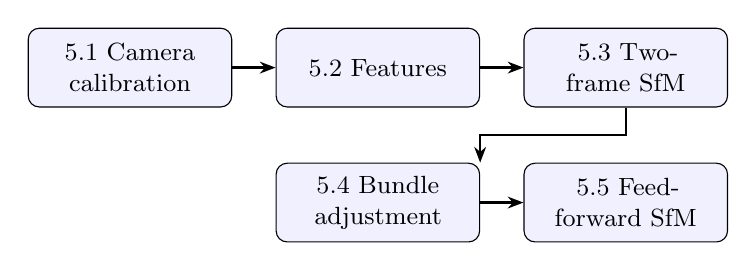
\begin{tikzpicture}[node distance=0.55cm,every node/.style={font=\small},
 box/.style={draw,rounded corners,fill=blue!6,minimum height=1.0cm,text width=2.35cm,align=center},
 arr/.style={-{Stealth[length=2mm]},thick}]
\node[box] (a) {5.1 Camera calibration};
\node[box,right=of a] (b) {5.2 Features};
\node[box,right=of b] (c) {5.3 Two-frame SfM};
\node[box,below=0.7cm of b] (d) {5.4 Bundle adjustment};
\node[box,right=of d] (e) {5.5 Feed-forward SfM};
\draw[arr] (a)--(b); \draw[arr] (b)--(c); \draw[arr] (c.south)--++(0,-0.35)-|(d.north east) ;
\draw[arr] (d)--(e);
\end{tikzpicture}
\end{center}

\paragraph{Learning objectives (slide 2).}
\begin{enumerate}
\item Derive the epipolar constraint, estimate the essential matrix from correspondences, recover the
 relative pose up to scale, and triangulate a point from two views.
\item Formulate bundle adjustment as least squares over poses in $\SE$ and 3D points, solve it with
 Gauss--Newton and the Schur complement, and describe the stages of incremental SfM.
\item Explain how a feed-forward transformer predicts cameras, depth, point maps and tracks, and how
 bundle adjustment refines them.
\end{enumerate}

\paragraph{Notation used throughout.}
\begin{center}
\begin{tabular}{@{}ll@{}}
\toprule
Symbol & Meaning\\
\midrule
$\xb=(x,y,1)\tr$ & homogeneous pixel coordinates\\
$\xt=\bm K^{-1}\xb$ & local ray direction of a pixel (calibrated camera)\\
$\bm R,\bm t$, $\bm T=[\bm R|\bm t]\in\SE$ & rotation, translation, pose (world $\to$ camera)\\
$\sk{\bm t}$ & skew-symmetric matrix with $\sk{\bm t}\bm v=\bm t\times\bm v$\\
$\E=\sk{\bm t}\bm R$, $\Fm=\bm K_2^{-\mathsf T}\E\bm K_1^{-1}$ & essential / fundamental matrix\\
$\bm x^w_p$, $\bm x^s_{ip}$ & 3D world point $p$, its observation in image $i$\\
$\propto$ & equality up to a nonzero scale factor\\
\bottomrule
\end{tabular}
\end{center}

%%%%%%%%%%%%%%%%%%%%%%%%%%%%%%%%%%%%%%%%%%%%%%%%%%%%%%%%%%%%%%%%%%%%%%
\section{Camera Calibration \slr{3--7}}

\subsection{What calibration is and how it is done \slr{4--7}}
\emph{Camera calibration} is the process of finding the intrinsic and extrinsic parameters of a
camera. Most commonly a \emph{known calibration target} (an image or a checkerboard) is used.

\begin{definition}{Pinhole camera with intrinsics and extrinsics}{pinhole}
A world point $\bm x^w\in\R^3$ is mapped to a pixel by
\[
\lambda\,\xb=\bm K\,[\bm R\,|\,\bm t]\begin{pmatrix}\bm x^w\\1\end{pmatrix},\qquad
\bm K=\begin{pmatrix}f_x&s&c_x\\0&f_y&c_y\\0&0&1\end{pmatrix},
\]
where $\bm K$ holds the \emph{intrinsics} (focal lengths $f_x,f_y$ in pixels, skew $s$, principal
point $(c_x,c_y)$) and $[\bm R|\bm t]\in\SE$ are the \emph{extrinsics}, i.e.\ the camera pose.
Lens \emph{distortion} (e.g.\ radial, $\bm x_d=\bm x\,(1+k_1r^2+k_2r^4)$ with $r=\norm{\bm x}$ in
normalized coordinates) is modelled by extra parameters applied before $\bm K$.
\end{definition}

\begin{intuition}
$\bm K$ says how the metric ray through the pinhole is converted to pixels; $[\bm R|\bm t]$ says where the
camera sits in the world. Calibration is an inverse problem: we look at something whose geometry we
know perfectly (the target) and ask which camera would have produced those pixels.
\end{intuition}

The procedure on slides 4--7 has four stages (Fig.~\ref{fig:calibflow}):
\begin{enumerate}
\item the known target is \textbf{captured in different poses} (slide 5);
\item \textbf{features} (e.g.\ corners) on the target are detected in the images (slide 6);
\item a \textbf{closed-form solution} initializes all parameters except the distortion parameters;
\item a \textbf{non-linear optimization} of all parameters minimizes the reprojection errors
 (slide 7), jointly over intrinsics and extrinsics (=poses).
\end{enumerate}

\begin{figure}[H]
\centering
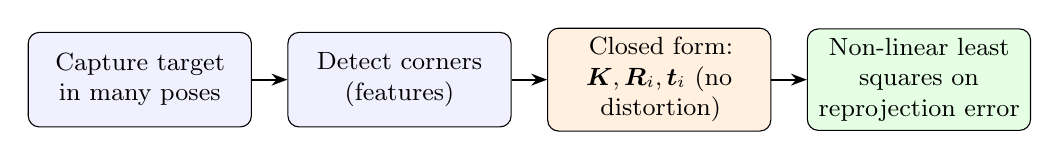
\begin{tikzpicture}[node distance=0.45cm,every node/.style={font=\small},
 box/.style={draw,rounded corners,fill=blue!6,minimum height=1.2cm,text width=2.6cm,align=center},
 arr/.style={-{Stealth[length=2mm]},thick}]
\node[box] (a) {Capture target in many poses};
\node[box,right=of a] (b) {Detect corners (features)};
\node[box,right=of b,fill=orange!12] (c) {Closed form: $\bm K,\bm R_i,\bm t_i$ (no distortion)};
\node[box,right=of c,fill=green!10] (d) {Non-linear least squares on reprojection error};
\draw[arr](a)--(b);\draw[arr](b)--(c);\draw[arr](c)--(d);
\end{tikzpicture}
\caption{The calibration pipeline of Zhang (2000), redrawn from the description on slides 4--7.}
\label{fig:calibflow}
\end{figure}

\imgph[3.2cm]{4}{A known calibration target held in front of several cameras (multi-camera calibration setup).}
\imgph[3.2cm]{5}{The calibration checkerboard captured in 20 different poses.}
\imgph[3.2cm]{6}{Corners detected on the target (red crosses, blue squares: extracted corners).}
\imgph[3.2cm]{7}{Recovered extrinsic parameters: the target planes in the camera frame after joint optimization (Zhang, TPAMI 2000).}

\begin{theorem}{Zhang's constraints from a plane}{zhang}
Let the target lie in the plane $Z=0$ of the world, so a target point is $(X,Y,0)$. The homography
$\bm H=[\bm h_1\ \bm h_2\ \bm h_3]$ mapping target coordinates $(X,Y,1)\tr$ to pixels satisfies
$\bm H=\lambda\bm K[\bm r_1\ \bm r_2\ \bm t]$. With $\bm B=\bm K^{-\mathsf T}\bm K^{-1}$ (symmetric,
positive definite) every view yields the two linear equations in $\bm B$
\[
\bm h_1\tr\bm B\,\bm h_2=0,\qquad \bm h_1\tr\bm B\,\bm h_1=\bm h_2\tr\bm B\,\bm h_2 .
\]
\end{theorem}
\begin{proof}
For $Z=0$ the column $\bm r_3$ is multiplied by zero, so $\lambda\xb=\bm K[\bm r_1\ \bm r_2\ \bm t](X,Y,1)\tr$,
which gives $\bm H$. From $\bm h_i=\lambda\bm K\bm r_i$ we get $\bm r_i=\lambda^{-1}\bm K^{-1}\bm h_i$ for $i=1,2$.
Rotation columns are orthogonal and unit norm: $\bm r_1\tr\bm r_2=0$ gives
$\bm h_1\tr\bm K^{-\mathsf T}\bm K^{-1}\bm h_2=0$ and $\bm r_1\tr\bm r_1=\bm r_2\tr\bm r_2$ gives the second equation.
\end{proof}

\begin{intuition}
A rotation matrix has two ``rules'': its columns are perpendicular and equally long. A single view of a
flat board gives a homography, and those two rules, pushed through the unknown $\bm K$, become two
equations on $\bm B$ (which encodes $\bm K$). The board in one pose cannot tell you everything; a tilted
board in a different pose tells you something new. That is why the target is captured in different poses.
\end{intuition}

\paragraph{Counting.} $\bm B$ is symmetric, so it has 6 entries; it is defined up to scale, so 5 unknowns
(matching the 5 intrinsics of $\bm K$). Each view gives 2 equations, hence $\ge 3$ views for a general $\bm K$ (or 2 views
if the skew $s=0$ is assumed).

\begin{algorithm}{Zhang's calibration}{zhangalg}
\begin{enumerate}[nosep]
\item For each view $j$ estimate the homography $\bm H_j$ from the detected corners (DLT, as for homography
 estimation in lecture 01).
\item Stack the two equations of Thm.~\ref{thm:zhang} for all views as $\bm V\bm b=0$ and take the right singular
 vector of the smallest singular value; recover $\bm K$ from $\bm b$.
\item For every view: $\lambda=1/\norm{\bm K^{-1}\bm h_1}$, $\bm r_1=\lambda\bm K^{-1}\bm h_1$,
 $\bm r_2=\lambda\bm K^{-1}\bm h_2$, $\bm r_3=\bm r_1\times\bm r_2$, $\bm t=\lambda\bm K^{-1}\bm h_3$.
 (Project $[\bm r_1\bm r_2\bm r_3]$ to the closest rotation with an SVD.) Distortion is initialized to zero.
\item Refine all parameters jointly by minimizing the reprojection error
 $\sum_{j,m}\norm{\xb_{jm}-\hat\pi(\bm K,\bm k,\bm R_j,\bm t_j,\bm X_m)}^2$ with a non-linear least-squares solver
 (Levenberg--Marquardt).
\end{enumerate}
\end{algorithm}

\begin{intuition}
Steps 1--3 are cheap and linear but ignore noise statistics and distortion; they only have to be
\emph{good enough to start}. Step 4 is the honest estimator. This ``closed form to initialize, non-linear
least squares to polish'' pattern returns again in bundle adjustment (Section~5.4).
\end{intuition}

\begin{example}{Size of a calibration problem (illustrative numbers)}{calibsize}
A $9\times 6$ checkerboard (54 inner corners) seen in 20 views gives $2\cdot54\cdot20=2160$ scalar
residuals. The unknowns are 5 intrinsics, 2 distortion coefficients and $6\cdot20=120$ pose parameters: $127$ in total.
The problem is hugely over-determined, which is what makes it accurate.
\end{example}

%%%%%%%%%%%%%%%%%%%%%%%%%%%%%%%%%%%%%%%%%%%%%%%%%%%%%%%%%%%%%%%%%%%%%%
\section{Feature Detection and Description \slr{8--20}}

\subsection{Point Features \slr{9--11}}
\imgph[3.4cm]{9}{Two views of the same mountain scene; red boxes mark patches that are flat sky (uninformative), an edge, and a distinctive corner-like region (image credit: R.~Szeliski).}

\begin{definition}{Point feature}{pointfeat}
A point feature is a pair $(\bm k,\bm f)$: a \emph{keypoint} $\bm k=(x,y)\tr\in\R^2$, the pixel location of a
salient region, and a \emph{descriptor} $\bm f\in\R^D$ that describes the appearance of the image around $\bm k$.
An image yields a set of $M$ features $\{(\bm k_j,\bm f_j)\}_{j=1}^M$. Two features $(\bm k,\bm f)$ and
$(\bm k',\bm f')$ in two images \emph{match} when their descriptors are close, i.e.\ $\norm{\bm f-\bm f'}$ is small.
\end{definition}

\begin{intuition}
Think of a descriptor as a ``fingerprint'' of a patch. A flat piece of sky has a fingerprint that
matches thousands of other patches (useless), whereas the tip of a mountain has a unique one. Point features describe local
salient regions, they can be used to describe and match images from different viewpoints, and they
form the basis of the sparse 3D reconstruction methods of this lecture.
\end{intuition}

The requirements (slide 11): features should be \textbf{invariant} to perspective effects and illumination, and the same
3D point should have \textbf{similar vectors independent of pose/viewpoint}. Plain RGB/intensity patches
do not have this property, so we need something better.

\imgph[3.4cm]{11}{Object recognition with local scale-invariant features: SIFT patches on three known products are found in a cluttered scene (Lowe, ICCV 1999).}

\subsection{Scale Invariant Feature Transform (SIFT) \slr{12--15}}
\paragraph{Detection (slide 12).} SIFT builds a \emph{scale space} by iteratively filtering the image with a Gaussian.
Adjacent scales are subtracted, yielding \emph{Difference of Gaussian} (DoG) images; interest points
(=blobs) are detected as extrema in the resulting scale space (Fig.~\ref{fig:siftscale}).

\begin{figure}[H]
\centering
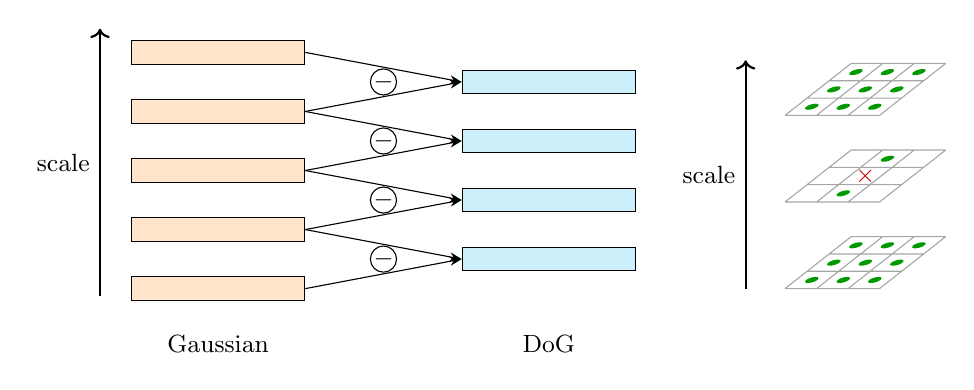
\begin{tikzpicture}[every node/.style={font=\small}]
\foreach \i in {0,...,4}{\node[draw,fill=orange!20,minimum width=2.2cm,minimum height=0.3cm] (g\i) at (0,0.75*\i) {};}
\foreach \i in {0,...,3}{\node[draw,fill=cyan!20,minimum width=2.2cm,minimum height=0.3cm] (d\i) at (4.2,0.75*\i+0.375) {};}
\foreach \i [evaluate=\j as \j using int(\i+1)] in {0,...,3}{
 \draw[-{Stealth[length=1.5mm]}] (g\i.east)--(d\i.west);
 \draw[-{Stealth[length=1.5mm]}] (g\j.east)--(d\i.west);
 \node[draw,circle,fill=white,inner sep=0pt,minimum size=3mm] at (2.1,0.75*\i+0.375) {$-$};}
\node at (0,-0.7) {Gaussian};\node at (4.2,-0.7) {DoG};
\draw[->,thick] (-1.5,-0.1)--(-1.5,3.3) node[midway,left]{scale};
% neighbourhood
\begin{scope}[shift={(7.2,0)}]
\foreach \l/\y in {0/0,1/1.1,2/2.2}{
 \begin{scope}[shift={(0,\y)}, yscale=0.55, xslant=0.7]
 \draw[step=0.4,gray!70] (0,0) grid (1.2,1.2);
 \foreach \a in {0,1,2}{\foreach \b in {0,1,2}{
   \ifnum\l=1 \ifnum\a=1 \ifnum\b=1 \else \fill[green!60!black] (0.4*\a+0.2,0.4*\b+0.2) circle (2pt);\fi\fi\else \fill[green!60!black] (0.4*\a+0.2,0.4*\b+0.2) circle (2pt);\fi}}
 \ifnum\l=1 \node[red!80!black] at (0.6,0.6) {$\times$}; \fi
 \end{scope}}
\draw[->,thick] (-0.5,0)--(-0.5,2.9) node[midway,left]{scale};
\end{scope}
\end{tikzpicture}
\caption{Left: first octave of the Gaussian scale space and the DoG images obtained by subtracting neighbouring scales.
Right: a candidate (red cross) is kept only if it is larger or smaller than all its 26 neighbours in space and scale (green).}
\label{fig:siftscale}
\end{figure}

\begin{proposition}{DoG approximates the scale-normalized Laplacian}{dog}
Let $G(\bm x,\sigma)=\frac1{2\pi\sigma^2}e^{-\norm{\bm x}^2/2\sigma^2}$. Then $\partial G/\partial\sigma=\sigma\nabla^2G$ and,
for a scale ratio $k$ close to 1,
\[
G(\bm x,k\sigma)-G(\bm x,\sigma)\;\approx\;(k-1)\,\sigma^2\nabla^2G(\bm x,\sigma).
\]
\end{proposition}
\begin{proof}
$G$ solves the heat equation $\partial G/\partial(\sigma^2)=\tfrac12\nabla^2G$, i.e.\ $\partial G/\partial\sigma=\sigma\nabla^2G$.
A finite difference in $\sigma$ gives $G(k\sigma)-G(\sigma)\approx(k\sigma-\sigma)\,\partial G/\partial\sigma=(k-1)\sigma^2\nabla^2G$.
\end{proof}

\begin{intuition}
Subtracting two slightly different blurs is a cheap way to compute a blob detector (the Laplacian). Multiplying by $\sigma^2$ makes
its response comparable across scales: a big blob at a coarse scale gives the same peak value as a small blob at a fine
scale, so extrema over (position, scale) find blobs together with their size. That is where scale invariance comes from.
\end{intuition}

\paragraph{Description (slide 13).}
SIFT \textbf{rotates} the descriptor to \textbf{align with the dominant gradient orientation}; \textbf{gradient histograms} are computed
for local sub-regions; all histograms are concatenated and normalized to form a \textbf{128D feature vector}.

\begin{figure}[H]
\centering
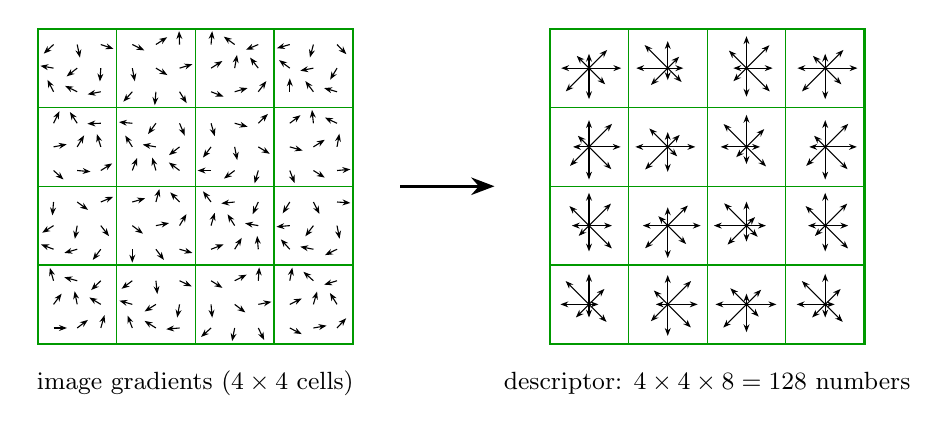
\begin{tikzpicture}[every node/.style={font=\small}]
% gradient samples
\draw[green!60!black,thick] (0,0) rectangle (4,4);
\foreach \i in {0,...,3}{\foreach \j in {0,...,3}{
  \draw[green!60!black] (\i,\j) rectangle (\i+1,\j+1);
  \foreach \u in {0,...,2}{\foreach \v in {0,...,2}{
    \pgfmathsetmacro{\ang}{mod(37*(\i*3+\u)+53*(\j*3+\v)+11*\u*\v,360)}
    \draw[-{Stealth[length=1mm]}] (\i+0.2+0.3*\u,\j+0.2+0.3*\v)--++(\ang:0.17);}}}}
\node at (2,-0.5) {image gradients ($4\times4$ cells)};
\draw[-{Stealth},very thick] (4.6,2)--(5.8,2);
% histograms
\begin{scope}[shift={(6.5,0)}]
\draw[green!60!black,thick] (0,0) rectangle (4,4);
\foreach \i in {0,...,3}{\foreach \j in {0,...,3}{
  \draw[green!60!black] (\i,\j) rectangle (\i+1,\j+1);
  \foreach \a in {0,45,...,315}{
    \pgfmathsetmacro{\len}{0.12+0.3*abs(sin(\a*0.7+\i*60+\j*35))}
    \draw[-{Stealth[length=1mm]}] (\i+0.5,\j+0.5)--++(\a:\len);}}}
\node at (2,-0.5) {descriptor: $4\times4\times8=128$ numbers};
\end{scope}
\end{tikzpicture}
\caption{Schematic of the SIFT descriptor: the gradients around the keypoint (after rotating to the dominant orientation) are
pooled into an orientation histogram with 8 bins per cell; $4\times4$ cells give a 128D vector.}
\end{figure}

\begin{intuition}
Histograms of gradient \emph{directions} throw away exact pixel positions inside each cell (robust to small shifts) but keep
the coarse layout (distinctive). Rotating to the dominant orientation removes the camera's in-plane rotation; normalizing the vector
removes affine illumination changes (gain).
\end{intuition}

\begin{beyond}
In Lowe's implementation, the vector is normalized, entries are clipped at $0.2$, and it is re-normalized, which reduces the
influence of non-linear illumination effects. The slide shows a $2\times2$ grid only for drawing convenience.
\end{beyond}

\subsection{Matching features \slr{14--15}}
Many algorithms exist (SIFT, SURF, U-SURF, BRISK, ORB, FAST and learned ones such as SuperPoint). SIFT was a seminal work thanks to its
invariance and robustness and enabled large-scale SfM; despite being 20 years old it is still used, e.g.\ in COLMAP.
Correspondences are retrieved by efficient nearest-neighbour search. Ambiguous matches are filtered with the \textbf{ratio test}:
compute the distance to the closest neighbour divided by the distance to the second closest; a large ratio ($>0.8$) indicates that the
match might not be correct.

\begin{definition}{Lowe's ratio test}{ratio}
For a query descriptor $\bm f$ with nearest neighbours $\bm f'_{(1)},\bm f'_{(2)}$ in the other image, accept the match
$\bm f\leftrightarrow\bm f'_{(1)}$ iff $\;\dfrac{\norm{\bm f-\bm f'_{(1)}}}{\norm{\bm f-\bm f'_{(2)}}}<\tau$, with typically $\tau=0.8$.
\end{definition}

\begin{figure}[H]
\centering
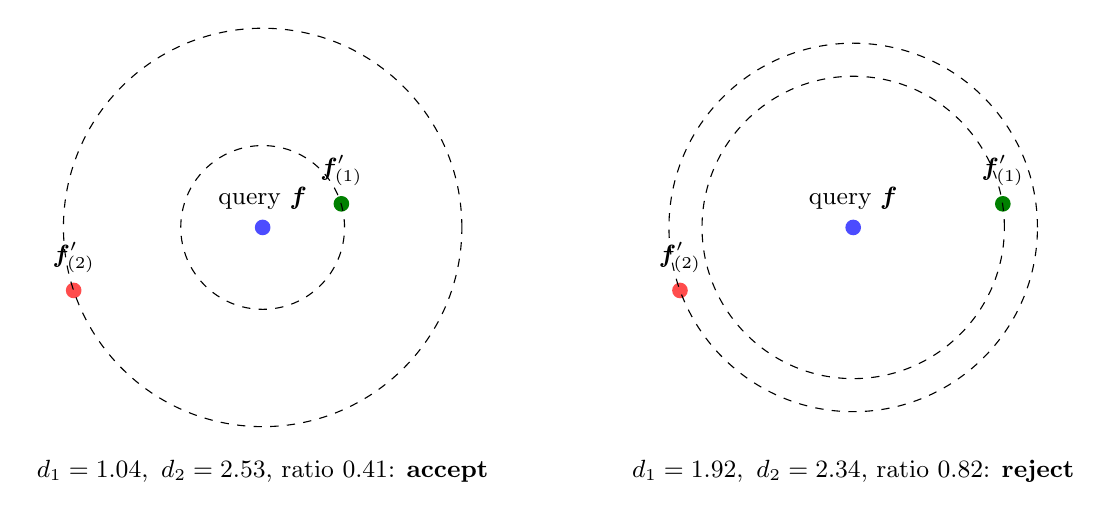
\begin{tikzpicture}[every node/.style={font=\small}]
\begin{scope}
\node[circle,fill=blue!70,inner sep=2pt,label=above:{query $\bm f$}] (q) at (0,0) {};
\node[circle,fill=green!50!black,inner sep=2pt,label=above:{$\bm f'_{(1)}$}] (a) at (1.0,0.3) {};
\node[circle,fill=red!70,inner sep=2pt,label=above:{$\bm f'_{(2)}$}] (b) at (-2.4,-0.8) {};
\draw[dashed] (q) circle (1.04); \draw[dashed] (q) circle (2.53);
\node at (0,-3.1) {$d_1=1.04,\ d_2=2.53$, ratio $0.41$: \textbf{accept}};
\end{scope}
\begin{scope}[shift={(7.5,0)}]
\node[circle,fill=blue!70,inner sep=2pt,label=above:{query $\bm f$}] (q) at (0,0) {};
\node[circle,fill=green!50!black,inner sep=2pt,label=above:{$\bm f'_{(1)}$}] (a) at (1.9,0.3) {};
\node[circle,fill=red!70,inner sep=2pt,label=above:{$\bm f'_{(2)}$}] (b) at (-2.2,-0.8) {};
\draw[dashed] (q) circle (1.92); \draw[dashed] (q) circle (2.34);
\node at (0,-3.1) {$d_1=1.92,\ d_2=2.34$, ratio $0.82$: \textbf{reject}};
\end{scope}
\end{tikzpicture}
\caption{Toy example in a 2D descriptor space. If the best match is not clearly better than the runner-up, the match is ambiguous.}
\end{figure}

\begin{intuition}
If I ask ``who is my best friend?'' and the answer is ``person A, and person B is almost as close'', I should not
trust the answer. The ratio test measures that gap. With ratio $0.41$ the closest descriptor is more than twice as close as
the next; with ratio $0.82$ it is basically a coin flip between two candidates (e.g.\ a repeated window on a facade).
\end{intuition}

\imgph[3.8cm]{15}{Two images of Notre-Dame with SIFT correspondences (green: correct, red: wrong) (image credits: J.~Hays).}

\subsection{SuperPoint: Learned Interest Points and Descriptors \slr{16--20}}
\paragraph{Idea (slide 16).} A fully convolutional network computes interest points and their descriptors in one forward pass over the
full image. Training is \textbf{self-supervised} in three stages (Fig.~\ref{fig:sp3}): (a) a base detector, MagicPoint, is trained on rendered
shapes whose corners are known; (b) it labels real, unlabeled images by Homographic Adaptation; (c) detector and descriptor are trained jointly on
image pairs related by a known homography. Runtime: about $13$\,ms for a $480\times640$ image on one Titan~X GPU (about 70 fps).

\begin{figure}[H]
\centering
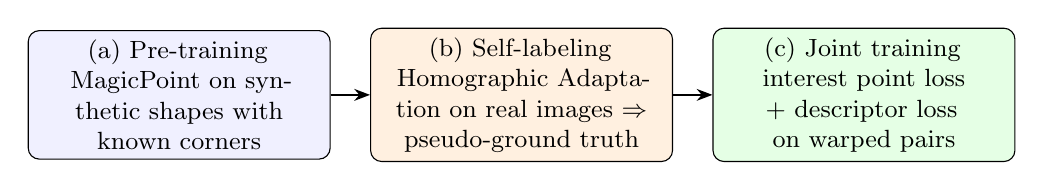
\begin{tikzpicture}[node distance=0.5cm,every node/.style={font=\small},
 box/.style={draw,rounded corners,fill=blue!6,minimum height=1.3cm,text width=3.6cm,align=center},
 arr/.style={-{Stealth[length=2mm]},thick}]
\node[box] (a) {(a) Pre-training\\ MagicPoint on synthetic shapes with known corners};
\node[box,right=of a,fill=orange!12] (b) {(b) Self-labeling\\ Homographic Adaptation on real images $\Rightarrow$ pseudo-ground truth};
\node[box,right=of b,fill=green!10] (c) {(c) Joint training\\ interest point loss + descriptor loss on warped pairs};
\draw[arr](a)--(b);\draw[arr](b)--(c);
\end{tikzpicture}
\caption{The three SuperPoint training stages (slide 16).}\label{fig:sp3}
\end{figure}

\paragraph{Base detector and training details (slide 17).}
MagicPoint is trained for 200,000 iterations on \emph{Synthetic Shapes} (quads, triangles, cubes, stars, lines, checkerboards, quad grids),
rendered on the fly so that no image is seen twice. Pseudo-ground truth: 80,000 MS-COCO images, grayscale, $240\times320$, Homographic
Adaptation with $N_h=100$, run twice. Joint training: one random homography per image (milder than in adaptation), cross-entropy for interest
points, a hinge loss for descriptors. Optimization: batch size 32, Adam with learning rate $10^{-3}$, augmentation (Gaussian noise, motion blur,
brightness), descriptor length $D=256$.

\imgph[3.2cm]{17}{Left: Synthetic Shapes with known corners. Right: MagicPoint against FAST, Harris and Shi--Tomasi corners on noisy images.}

\paragraph{Homographic Adaptation (slide 18).}
\begin{definition}{Covariant detector and Homographic Adaptation}{homadapt}
Let $f_\theta$ map an image to a heatmap of interest points and let $\tilde{\bm H}(\cdot)$ denote warping an image or heatmap by the homography $\tilde{\bm H}$.
$f_\theta$ is \emph{covariant} if $f_\theta(\tilde{\bm H}(\bm I))=\tilde{\bm H}(f_\theta(\bm I))$. Homographic Adaptation computes the label heatmap
\[
\hat F(\bm I)=\frac1{N_h}\sum_{i=1}^{N_h}\tilde{\bm H}_i^{-1}\bigl(f_\theta(\tilde{\bm H}_i(\bm I))\bigr),
\]
with random homographies $\tilde{\bm H}_i$ and $N_h=100$ warps.
\end{definition}

\begin{lemma}{Averaging over warps}{avgwarp}
If $f_\theta$ is exactly covariant, then $\hat F(\bm I)=f_\theta(\bm I)$ for every $N_h$.
\end{lemma}
\begin{proof}
Each term equals $\tilde{\bm H}_i^{-1}\bigl(\tilde{\bm H}_i(f_\theta(\bm I))\bigr)=f_\theta(\bm I)$, and the mean of $N_h$ equal terms is that term.
\end{proof}

\begin{intuition}
A real network is only approximately covariant: it finds a corner from one viewpoint and misses it from another. Looking at the image through
100 different warps and voting (after un-warping the heatmaps) keeps the points the detector finds \emph{consistently} and averages out accidental
misses, so the labels impose covariance on the training data. The labels are generated on everyday photographs with no annotation of
interest points: that is what ``self-supervised'' means here.
\end{intuition}

\begin{figure}[H]
\centering
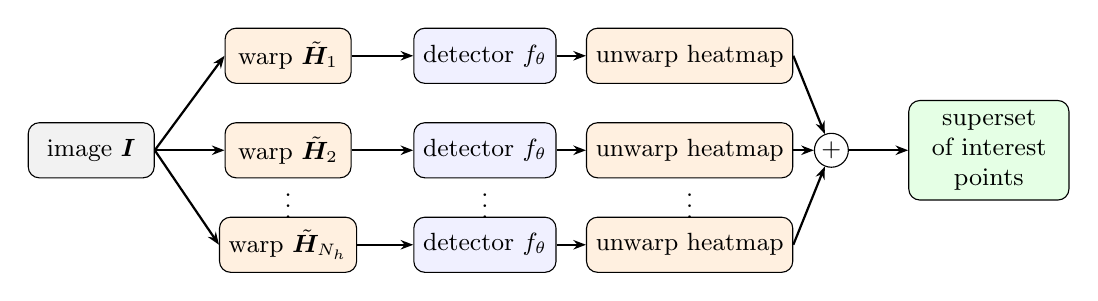
\begin{tikzpicture}[node distance=0.35cm,every node/.style={font=\small},
 s/.style={draw,rounded corners,minimum height=0.7cm,minimum width=1.6cm,align=center,fill=blue!6},
 arr/.style={-{Stealth[length=1.6mm]},thick}]
\node[s,fill=gray!10] (im) at (0,0) {image $\bm I$};
\foreach \k/\lab/\y in {1/{$\tilde{\bm H}_1$}/1.2,2/{$\tilde{\bm H}_2$}/0,3/{$\tilde{\bm H}_{N_h}$}/-1.2}{
 \node[s,fill=orange!12] (h\k) at (2.5,\y) {warp \lab};
 \node[s] (d\k) at (5.0,\y) {detector $f_\theta$};
 \node[s,fill=orange!12] (u\k) at (7.6,\y) {unwarp heatmap};
 \draw[arr] (im.east)--(h\k.west); \draw[arr](h\k)--(d\k); \draw[arr](d\k)--(u\k);}
\node at (2.5,-0.6) {$\vdots$};\node at (5,-0.6) {$\vdots$};\node at (7.6,-0.6) {$\vdots$};
\node[draw,circle,fill=white,inner sep=1pt] (sum) at (9.4,0) {$+$};
\foreach \k in {1,2,3}{\draw[arr](u\k.east)--(sum);}
\node[s,fill=green!10,text width=1.8cm] (sup) at (11.4,0) {superset of interest points};
\draw[arr](sum)--(sup);
\end{tikzpicture}
\caption{Homographic Adaptation (redrawn from slide 18): detect on warped copies, un-warp, average, and extract the pseudo-ground-truth points.}
\end{figure}

\paragraph{Architecture (slide 19).}
The encoder consists of eight $3\times3$ convolutions and three $2\times2$ max pools, hence one cell $c$ per $8\times8$ pixels. Two heads share it
(Fig.~\ref{fig:spnet}).
\begin{itemize}
\item \textbf{Keypoint head:} $\bm S\in\R^{H/8\times W/8\times 65}$. Each cell is classified into 65 classes: one per pixel and one for ``no keypoint''
 (the 65th class). The loss is the cross-entropy against the pseudo-ground-truth label $y_c$, averaged over the $HW/64$ cells:
 \[
 \mathcal L_p=-\frac{64}{HW}\sum_c\log\frac{\exp\bm S[c,y_c]}{\sum_{j=1}^{65}\exp\bm S[c,j]} .
 \]
\item \textbf{Descriptor head:} $\bm F\in\R^{H/8\times W/8\times256}$, one unit-length descriptor $\bm f\in\R^{256}$ per cell, interpolated at each
 keypoint $\bm k$ (bi-cubic interpolation, L2 normalization).
\item \textbf{Descriptor loss:} over all pairs of cells of the two images, with $s=1$ if the homography maps one onto the other,
 \[
 s\,\max(0,\,1-\bm f\tr\bm f')+(1-s)\,\max(0,\,\bm f\tr\bm f'-0.2).
 \]
\end{itemize}
\emph{Self-supervision through known homography.}

\begin{figure}[H]
\centering
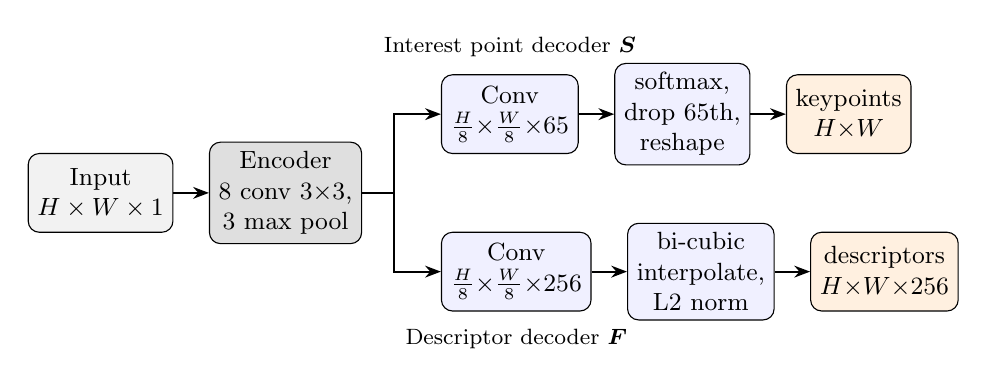
\begin{tikzpicture}[node distance=0.45cm,every node/.style={font=\small},
 b/.style={draw,rounded corners,fill=blue!6,minimum height=1cm,align=center},
 arr/.style={-{Stealth[length=2mm]},thick}]
\node[b,fill=gray!10] (in) {Input\\ $H\times W\times1$};
\node[b,right=of in,fill=gray!25] (enc) {Encoder\\ 8 conv $3{\times}3$,\\ 3 max pool};
\node[b,right=1.0cm of enc,yshift=1.0cm] (k) {Conv\\ $\frac H8{\times}\frac W8{\times}65$};
\node[b,right=of k] (sm) {softmax,\\ drop 65th,\\ reshape};
\node[b,right=of sm,fill=orange!12] (ko) {keypoints\\ $H{\times}W$};
\node[b,right=1.0cm of enc,yshift=-1.0cm] (d) {Conv\\ $\frac H8{\times}\frac W8{\times}256$};
\node[b,right=of d] (bc) {bi-cubic\\ interpolate,\\ L2 norm};
\node[b,right=of bc,fill=orange!12] (do) {descriptors\\ $H{\times}W{\times}256$};
\draw[arr](in)--(enc);\draw[arr](enc.east)--++(0.4,0)|-(k.west);\draw[arr](enc.east)--++(0.4,0)|-(d.west);
\draw[arr](k)--(sm);\draw[arr](sm)--(ko);\draw[arr](d)--(bc);\draw[arr](bc)--(do);
\node[above=0.1cm of k,font=\footnotesize] {Interest point decoder $\bm S$};
\node[below=0.1cm of d,font=\footnotesize] {Descriptor decoder $\bm F$};
\end{tikzpicture}
\caption{SuperPoint architecture (redrawn from slide 19).}\label{fig:spnet}
\end{figure}

\begin{example}{Tensor sizes for a $480\times640$ image}{spsize}
There are $60\times80=4800$ cells. The keypoint head outputs a $60\times80\times65$ tensor; after the softmax the dustbin channel is dropped and the
remaining $64$ channels are reshaped to $8\times8$ pixels, giving a full-resolution $480\times640$ heatmap. The descriptor head outputs
$60\times80\times256$, i.e.\ a coarse semi-dense grid of descriptors that is interpolated at the detected keypoints.
At 13\,ms per image this is $\approx 77$ frames per second (the slide quotes 70).
\end{example}

\begin{intuition}
Instead of asking ``is this pixel a corner?'' $480\times640$ times, the network asks each $8\times8$ cell ``which of your 64 pixels is the corner,
or is there none?''. That is a 65-way classification, solved with an ordinary softmax and cross-entropy. The descriptor loss pulls
descriptors of cells that the homography matches towards the same direction (dot product close to 1, margin 1) and pushes non-matching ones
apart (dot product below 0.2).
\end{intuition}

\paragraph{Results on HPatches (slide 20).} HPatches has 116 scenes, 57 with large illumination changes and 59 with large viewpoint changes; at most 1000 points
per method at $480\times640$.

\begin{table}[H]
\centering
\begin{tabular}{lccccccc}
\toprule
Method & $\varepsilon{=}1$ & $\varepsilon{=}3$ & $\varepsilon{=}5$ & Rep. & MLE$\downarrow$ & NN mAP & M.\ Score\\
\midrule
SuperPoint & 0.310 & \textbf{0.684} & \textbf{0.829} & 0.581 & 1.158 & \textbf{0.821} & \textbf{0.470}\\
LIFT & 0.284 & 0.598 & 0.717 & 0.449 & 1.102 & 0.664 & 0.315\\
SIFT & \textbf{0.424} & 0.676 & 0.759 & 0.495 & \textbf{0.833} & 0.694 & 0.313\\
ORB & 0.150 & 0.395 & 0.538 & \textbf{0.641} & 1.157 & 0.735 & 0.266\\
\bottomrule
\end{tabular}
\caption{HPatches. $\varepsilon{=}1,3,5$: share of image pairs whose estimated homography is correct within $\varepsilon$ pixels; Rep.: detector repeatability; MLE: mean
localization error in pixels (lower is better); NN mAP: mean average precision of nearest-neighbour descriptor matching; M.\ Score: matching score.}
\end{table}

\begin{figure}[H]
\centering
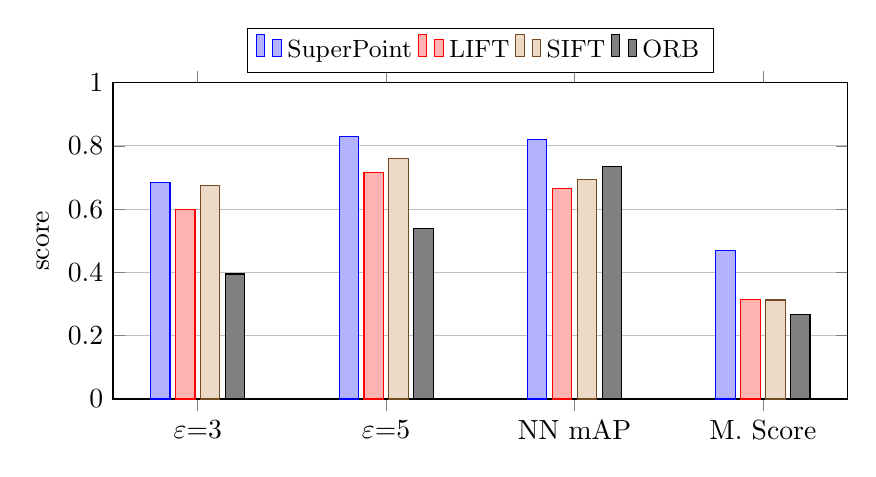
\begin{tikzpicture}
\begin{axis}[ybar,width=0.9\linewidth,height=5.6cm,bar width=7pt,ymin=0,ymax=1,
 symbolic x coords={eps3,eps5,NNmAP,MScore},xtick=data,
 xticklabels={$\varepsilon{=}3$,$\varepsilon{=}5$,NN mAP,M.\ Score},
 legend style={at={(0.5,1.03)},anchor=south,legend columns=4,font=\small},
 ylabel={score},enlarge x limits=0.15,ymajorgrids]
\addplot coordinates {(eps3,0.684)(eps5,0.829)(NNmAP,0.821)(MScore,0.470)};
\addplot coordinates {(eps3,0.598)(eps5,0.717)(NNmAP,0.664)(MScore,0.315)};
\addplot coordinates {(eps3,0.676)(eps5,0.759)(NNmAP,0.694)(MScore,0.313)};
\addplot coordinates {(eps3,0.395)(eps5,0.538)(NNmAP,0.735)(MScore,0.266)};
\legend{SuperPoint,LIFT,SIFT,ORB}
\end{axis}
\end{tikzpicture}
\caption{Selected HPatches metrics from the table (higher is better).}
\end{figure}

\begin{intuition}
SuperPoint wins on the metrics that depend on \emph{descriptors} and on how well matches are spread across the image (homography accuracy, NN mAP, matching score),
while SIFT is still best at sub-pixel \emph{localization} (lowest MLE) and at $\varepsilon{=}1$. On slide 20 the fourth row shows a failure of SuperPoint and LIFT
under an extreme in-plane rotation, a case absent from their training data: a learned method is only as invariant as its training augmentations.
\end{intuition}

\imgph[3.8cm]{20}{Qualitative matches of SuperPoint, LIFT, SIFT and ORB on six HPatches pairs (green: matches; the fourth row shows an extreme in-plane rotation).}
%%%%%%%%%%%%%%%%%%%%%%%%%%%%%%%%%%%%%%%%%%%%%%%%%%%%%%%%%%%%%%%%%%%%%%
\section{Two-Frame Structure-from-Motion \slr{21--35}}

\subsection{Epipolar Geometry \slr{22--23}}
\textbf{Goal:} recovery of camera pose (and 3D structure) from image correspondences. The required relationships are described by the two-view
\emph{epipolar geometry}.

\begin{itemize}
\item Let $\bm R$ and $\bm t$ denote the relative pose between two perspective cameras.
\item A 3D point $\bm x$ is projected to pixel $\xb_1$ in image 1 and to pixel $\xb_2$ in image 2.
\item The 3D point $\bm x$ and the two camera centers span the \textbf{epipolar plane}.
\item The correspondence of $\xb_1$ in image 2 must lie on the \textbf{epipolar line} $\tilde{\bm l}_2$ in image 2.
\item All epipolar lines pass through the \textbf{epipole}.
\end{itemize}

\begin{figure}[H]
\centering
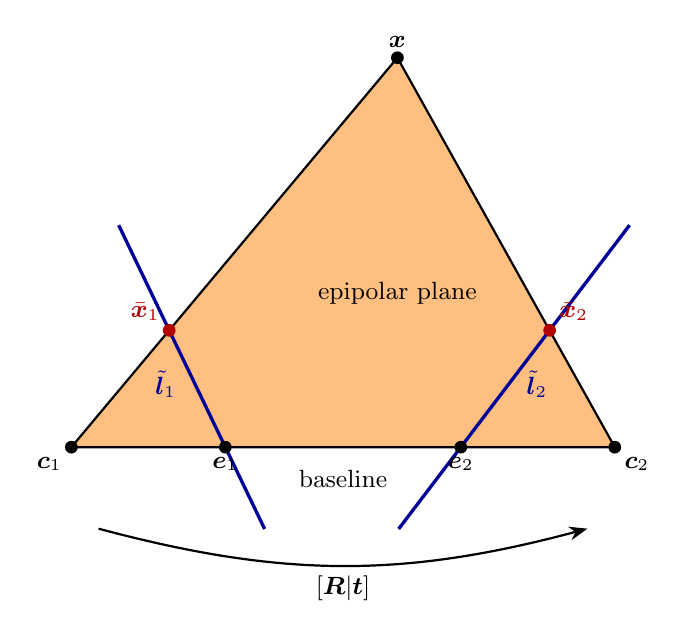
\begin{tikzpicture}[scale=1.15,every node/.style={font=\small}]
\coordinate (C1) at (0,0); \coordinate (C2) at (6,0); \coordinate (X) at (3.6,4.3);
\coordinate (x1) at ($(C1)!0.3!(X)$); \coordinate (x2) at ($(C2)!0.3!(X)$);
\coordinate (e1) at (1.7,0); \coordinate (e2) at (4.3,0);
\fill[orange!50] (C1)--(C2)--(X)--cycle;
\draw[thick] (C1)--(X)--(C2)--cycle;
% image planes (edge-on in the epipolar plane = epipolar lines)
\draw[very thick,blue!60!black] ($(e1)!-0.7!(x1)$)--($(e1)!1.9!(x1)$);
\draw[very thick,blue!60!black] ($(e2)!-0.7!(x2)$)--($(e2)!1.9!(x2)$);
\fill (C1) circle (2pt) node[below left]{$\bm c_1$}; \fill (C2) circle (2pt) node[below right]{$\bm c_2$};
\fill (X) circle (2pt) node[above]{$\bm x$};
\fill[red!70!black] (x1) circle (2pt) node[above left]{$\xb_1$};
\fill[red!70!black] (x2) circle (2pt) node[above right]{$\xb_2$};
\fill (e1) circle (2pt) node[below]{$\bm e_1$}; \fill (e2) circle (2pt) node[below]{$\bm e_2$};
\node[blue!60!black] at ($(e1)!0.5!(x1)+(-0.35,0.05)$) {$\tilde{\bm l}_1$};
\node[blue!60!black] at ($(e2)!0.5!(x2)+(0.35,0.05)$) {$\tilde{\bm l}_2$};
\node at (3.6,1.7) {epipolar plane};
\node at (3,-0.35) {baseline}; 
\draw[-{Stealth},thick] (0.3,-0.9) to[bend right=15] node[below]{$[\bm R|\bm t]$} (5.7,-0.9);
\end{tikzpicture}
\caption{Epipolar geometry (redrawn from slide 22). The image planes are drawn edge-on: their intersection with the epipolar plane is the epipolar line.}
\label{fig:epi}
\end{figure}

\begin{definition}{Epipolar plane, lines and epipoles}{epidef}
For a world point $\bm x$ and camera centers $\bm c_1,\bm c_2$, the \emph{epipolar plane} is the plane through $\bm x,\bm c_1,\bm c_2$. The \emph{baseline} is the line
$\bm c_1\bm c_2$. The \emph{epipole} $\bm e_i$ in image $i$ is the image of the other camera's center. The \emph{epipolar line} $\tilde{\bm l}_2$ of a pixel
$\xb_1$ is the intersection of the epipolar plane with image 2.
\end{definition}

\begin{intuition}
If I see a point in camera 1, I know it lies somewhere on the ray through $\bm c_1$ and $\xb_1$, but not how far. Camera 2 sees that whole ray as a
\emph{line}. So the 2D search for a match shrinks to a 1D search along the epipolar line (slide 30 shows this on real images). Because every ray passes through $\bm c_1$, all
the epipolar lines in image 2 pass through the projection of $\bm c_1$: the epipole.
\end{intuition}

\paragraph{Derivation of the epipolar constraint (slide 23).}
Let $\bm K_i$ be the calibration matrix of camera $i$, and $\xt_i=\bm K_i^{-1}\xb_i$ the local ray direction of pixel $\xb_i$ in camera $i$.

\begin{theorem}{Epipolar constraint}{epi}
Let $\bm x_2=\bm R\bm x_1+\bm t$ relate the coordinates of a 3D point in the two camera frames, and let $\E=\sk{\bm t}\bm R$ be the \emph{essential matrix}. Then
\[
\xt_2\tr\,\E\,\xt_1=0 .
\]
\end{theorem}
\begin{proof}
A point's camera coordinates are proportional to its ray direction: $\bm x_i\propto\xt_i$, say $\bm x_1=z_1\xt_1$, $\bm x_2=z_2\xt_2$. Then
$z_2\xt_2=z_1\bm R\xt_1+\bm t$, so $\xt_2\propto\bm R\xt_1+s\,\bm t$ for some scalar $s$ (slide: $\bm x_2\propto\bm R\xt_1+s\bm t$).
Taking the cross product with $\bm t$ (i.e.\ multiplying by $\sk{\bm t}$, which kills $\bm t$) gives $\sk{\bm t}\xt_2\propto\sk{\bm t}\bm R\xt_1$.
Taking the dot product with $\xt_2$: the left side is $\xt_2\tr\sk{\bm t}\xt_2=0$ because $\sk{\bm t}$ is skew-symmetric
($\bm v\tr\sk{\bm t}\bm v=\bm v\cdot(\bm t\times\bm v)=0$ by the triple product). Hence $\xt_2\tr\sk{\bm t}\bm R\xt_1=0$.
\end{proof}

\begin{intuition}
The three vectors $\xt_2$, $\bm R\xt_1$ and $\bm t$ all lie in the epipolar plane, so they are linearly dependent; their scalar triple product, $\xt_2\cdot(\bm t\times\bm R\xt_1)$, vanishes.
That is the entire constraint, written as a bilinear form $\xt_2\tr\E\,\xt_1=0$. It does not involve depth: we can test correspondences before knowing any 3D structure.
\end{intuition}

\begin{example}{The rectified stereo pair}{rectified}
Take $\bm R=\bm I$ and $\bm t=(1,0,0)\tr$ (a pure sideways shift of one unit). Then
$\E=\sk{\bm t}=\begin{psmallmatrix}0&0&0\\0&0&-1\\0&1&0\end{psmallmatrix}$ and for $\xt_i=(u_i,v_i,1)\tr$:
$\E\xt_1=(0,-1,v_1)\tr$, so $\xt_2\tr\E\xt_1=v_1-v_2=0$: corresponding points have the \textbf{same row}, i.e.\ epipolar lines are horizontal.
This is the stereo setting of lecture 04. With $\bm X=(X,Y,Z)\tr$ in camera 1, $u_1=X/Z$ and $u_2=(X+1)/Z$, so $u_2-u_1=1/Z$. If $u_1=0.1$ and $u_2=0.3$, then $Z=5$ (in units of the baseline).
\end{example}

\subsection{Structure of the Essential Matrix \slr{24}}
\begin{proposition}{Properties of $\E$}{eprops}
Let $\E=\sk{\bm t}\bm R$ with $\bm R\in\SO$ and $\bm t\neq0$. Then
\begin{enumerate}[nosep,label=(\roman*)]
\item $\E\E\tr=\sk{\bm t}\sk{\bm t}\tr=\norm{\bm t}^2\bm I-\bm t\bm t\tr$, hence the singular values of $\E$ are $(\norm{\bm t},\norm{\bm t},0)$ and $\E$ has rank 2;
\item $\bm t\tr\E=0$ (left null vector $\bm t\propto\bm e_2$) and $\E\,\bm R\tr\bm t=0$ (right null vector $\bm R\tr\bm t\propto\bm e_1$): each epipole is the image of the other camera's center;
\item $\E$ has 5 degrees of freedom: 3 for $\bm R$ and 3 for $\bm t$, minus one for the scale;
\item (scale ambiguity) scaling the scene and $\bm t$ by the same $\alpha$ leaves every image point unchanged, since $\alpha\bm x_2=\bm R(\alpha\bm x_1)+\alpha\bm t$. Hence $\norm{\bm t}$ cannot be observed and $\E$ is defined only up to scale, sign included.
\end{enumerate}
\end{proposition}
\begin{proof}
(i) $\E\E\tr=\sk{\bm t}\bm R\bm R\tr\sk{\bm t}\tr=\sk{\bm t}\sk{\bm t}\tr=\norm{\bm t}^2\bm I-\bm t\bm t\tr$, which has eigenvalues $\norm{\bm t}^2$ (twice, on $\bm t^\perp$) and $0$ (along $\bm t$).
(ii) $\bm t\tr\sk{\bm t}=-(\sk{\bm t}\bm t)\tr=0$, and $\E\bm R\tr\bm t=\sk{\bm t}\bm t=0$. The camera-1 center in camera-2 coordinates is $\bm R\cdot\bm 0+\bm t=\bm t$, so $\bm e_2\propto\bm t$; the camera-2 center in camera-1 coordinates is $-\bm R\tr\bm t$, so $\bm e_1\propto\bm R\tr\bm t$.
(iii) and (iv) follow from counting and from the displayed identity.
\end{proof}

\begin{intuition}
Rank 2 is the algebraic signature of ``all epipolar lines pass through one point'': the epipole is the null direction. The scale ambiguity is the same effect
that makes a photo of a model train indistinguishable from a photo of a real train: a single moving camera can recover the \emph{shape} of the scene and its \emph{motion direction}, never the absolute size, unless
something metric (a known length, an IMU, a stereo baseline) is available.
\end{intuition}

\begin{theorem}{Characterization of essential matrices}{echar}
A real $3\times3$ matrix is an essential matrix (up to scale) iff its SVD has the form $\bm U\diag(\sigma,\sigma,0)\bm V\tr$ with $\sigma>0$.
\end{theorem}
\begin{proof}
($\Rightarrow$) is Prop.~\ref{prop:eprops}(i). ($\Leftarrow$) Normalize $\sigma=1$ and choose $\bm U,\bm V$ with $\det=+1$ (flip the sign of the third column if needed: this does not change the
matrix because $\sigma_3=0$). Theorem~\ref{thm:decomp} below shows $\bm U\diag(1,1,0)\bm V\tr=\sk{\bm u_3}\bm R$ with $\bm R=\bm U\bm W\tr\bm V\tr\in\SO$.
\end{proof}

\subsection{Estimating the Essential Matrix: the 8-point algorithm \slr{25}}
Each correspondence $\xt_1=(x_1,y_1,1)\tr,\ \xt_2=(x_2,y_2,1)\tr$ gives one \emph{linear} equation in the nine entries of $\E$. Stacking the rows of a matrix into a vector,
\[
\xt_2\tr\E\xt_1=\vecop\bigl(\xt_2\tr\E\xt_1\bigr)=\bigl(\xt_1\otimes\xt_2\bigr)\tr\vecop(\E)=\bm a\tr\vecop(\E)=0,
\]
\[
\bm a=(x_2x_1,\ x_2y_1,\ x_2,\ y_2x_1,\ y_2y_1,\ y_2,\ x_1,\ y_1,\ 1)\tr,\qquad \vecop(\E)=(e_{11},e_{12},\dots,e_{33})\tr .
\]

\begin{algorithm}{Normalized 8-point algorithm}{eightpt}
\begin{enumerate}[nosep]
\item (Normalization) Whiten the observations to zero mean and unit variance, because products of two measurements amplify noise unevenly (Hartley 1997).
\item Stack the rows $\bm a_i\tr$ of $N\ge8$ correspondences into $\bm A\in\R^{N\times9}$ and solve $\min\norm{\bm A\vecop(\E)}$ s.t.\ $\norm{\vecop(\E)}=1$:
 the solution is the last right singular vector of $\bm A$.
\item (Projection) The estimate is not an essential matrix when there is noise. Take its SVD $\bm U\diag(\sigma_1,\sigma_2,\sigma_3)\bm V\tr$; the closest essential matrix in the Frobenius norm has singular values $(\bar\sigma,\bar\sigma,0)$ with $\bar\sigma=(\sigma_1+\sigma_2)/2$.
 As the scale is free, take $\E=\bm U\diag(1,1,0)\bm V\tr$.
\item (Undo the normalization.)
\end{enumerate}
\end{algorithm}

\begin{intuition}
Eight equations for nine unknowns defined up to scale: that is the minimal linear count. The $\bm A$-matrix is built so that $\bm A\vecop(\E)$ lists the ``epipolar errors'' of all correspondences, and the last singular vector is the $\E$ that makes their sum of squares smallest.
Step 3 then repairs the answer: the noisy $\E$ has three unequal singular values, so we average the top two and zero the third (which restores rank 2 and equal non-zero singular values).
\end{intuition}

\begin{lemma}{Projection onto essential matrices}{eproj}
Let $\bm M=\bm U\diag(\sigma_1,\sigma_2,\sigma_3)\bm V\tr$ with $\sigma_1\ge\sigma_2\ge\sigma_3\ge0$. Among matrices of the form $\bm U'\diag(\sigma,\sigma,0){\bm V'}\tr$ the one closest to $\bm M$ in the Frobenius norm is $\bm U\diag(\bar\sigma,\bar\sigma,0)\bm V\tr$ with $\bar\sigma=(\sigma_1+\sigma_2)/2$.
\end{lemma}
\begin{proof}[Sketch]
The Frobenius distance between matrices with singular values $\bm\sigma$ and $\bm\sigma'$ (sorted) is minimized by sharing the singular vectors and is then $\norm{\bm\sigma-\bm\sigma'}_2$ (Mirsky/von Neumann).
Minimizing $(\sigma_1-s)^2+(\sigma_2-s)^2+\sigma_3^2$ over $s$ gives $s=\bar\sigma$.
\end{proof}

\begin{intuition}
It is just ``the average is the best single number to replace two numbers in the least-squares sense''.
\end{intuition}

\paragraph{5-point solver.} The essential matrix has 5 degrees of freedom, hence 5 correspondences suffice (Nist\'er 2004). This minimal solver is what runs inside RANSAC in COLMAP and OpenCV.

\begin{beyond}
Minimal solvers are used inside RANSAC because the number of samples needed to hit an all-inlier set grows quickly with the sample size: with an inlier ratio $w=0.5$, the probability that a random sample of 8 is all inliers is $w^8\approx0.4\%$ while for 5 it is $w^5\approx3.1\%$, so about $8\times$ fewer iterations are needed.
\end{beyond}

\subsection{Decomposing the Essential Matrix \slr{26}}
Write $\E=\bm U\diag(1,1,0)\bm V\tr$, where $\bm u_k,\bm v_k$ denote the $k$-th columns of $\bm U,\bm V$ with $\det\bm U=\det\bm V=+1$. Let
\[
\bm W=\begin{pmatrix}0&-1&0\\1&0&0\\0&0&1\end{pmatrix}.
\]

\begin{theorem}{Four-fold ambiguity}{decomp}
$\E=\sk{\bm t}\bm R$ has exactly the four solutions (all up to scale)
\[
\bm R\in\{\bm U\bm W\bm V\tr,\ \bm U\bm W\tr\bm V\tr\},\qquad \bm t\in\{+\bm u_3,\,-\bm u_3\},\qquad\norm{\bm t}=1 .
\]
\end{theorem}
\begin{proof}
For a unit vector $\bm u_3=\bm U\bm e_3$ and $\det\bm U=1$ we have $\sk{\bm u_3}=\bm U\sk{\bm e_3}\bm U\tr$, and $\sk{\bm e_3}=\diag(1,1,0)\bm W$ (direct multiplication). Hence
$\sk{\bm u_3}=\bm U\diag(1,1,0)\bm W\bm U\tr$. Then
\[
\sk{\bm u_3}\,(\bm U\bm W\tr\bm V\tr)=\bm U\diag(1,1,0)\bm W\bm W\tr\bm V\tr=\E .
\]
Moreover, $\bm W^2=\diag(-1,-1,1)$ gives $\sk{\bm u_3}\,(\bm U\bm W\bm V\tr)=\bm U\diag(1,1,0)\bm W^2\bm V\tr=-\E$, i.e.\ $\sk{-\bm u_3}(\bm U\bm W\bm V\tr)=\E$.
So $(\bm U\bm W\tr\bm V\tr,+\bm u_3)$ and $(\bm U\bm W\bm V\tr,-\bm u_3)$ solve $\E=\sk{\bm t}\bm R$ exactly. Since $\E$ and $-\E$ are the same essential matrix (it is only defined up to scale, sign included), the pairs
$(\bm U\bm W\tr\bm V\tr,-\bm u_3)$ and $(\bm U\bm W\bm V\tr,+\bm u_3)$ are equally valid. The null space of $\sk{\bm t}$ is $\mathrm{span}(\bm t)$, which forces $\bm t\propto\bm u_3$, so there are no other solutions.
Finally $\bm R'=\bm U\bm W\bm V\tr=\bigl(\bm U\diag(-1,-1,1)\bm U\tr\bigr)\bm R$ with $\bm R=\bm U\bm W\tr\bm V\tr$: it differs from $\bm R$ by a half turn about $\bm u_3\propto\bm t$.
\end{proof}

\begin{intuition}
Two independent ambiguities hide in $\E$. (1) The \emph{sign} of $\bm t$: $\E$ and $-\E$ are the same constraint, so we cannot tell if the second camera is left or right of the first from the epipolar constraint alone.
(2) The \emph{twisted pair}: rotating camera 2 by $180^\circ$ about the baseline maps every epipolar plane to itself, so it also satisfies the constraint. $2\times2=4$ candidates; the geometry of the next slide tells us which one is real.
\end{intuition}

\subsection{Geometry of the Four Solutions \slr{27}}
With the true pose $(\bm R,\bm t)$ and the other rotation $\bm R'$, the four candidates place a scene point as drawn in Fig.~\ref{fig:four}.
\begin{itemize}
\item \textbf{Baseline reversal} ($\bm t\to-\bm t$, left to right in the slide): moves the center of camera 2, $-\bm R\tr\bm t$, to the other side of camera 1. Every point lands behind both cameras.
\item \textbf{Twisted pair} ($\bm R\to\bm R'$, top to bottom): $\bm R'^{\mathsf T}\bm R=\bm U\diag(-1,-1,1)\bm U\tr$, a half turn about $\bm u_3\propto\bm t$: camera 2 turns by $180^\circ$ about the baseline. Each point lands in front of one camera only.
\end{itemize}
Only $(\bm R,\bm t)$ puts the scene points in front of both cameras.

\newcommand{\camdraw}[3]{\begin{scope}[shift={(#1,#2)},rotate=#3]
 \fill[gray!25,draw=black] (0,0)--(-0.45,0.65)--(0.45,0.65)--cycle;
 \draw[-{Stealth},thick](0,0.65)--(0,1.25);\end{scope}}
\begin{figure}[H]
\centering
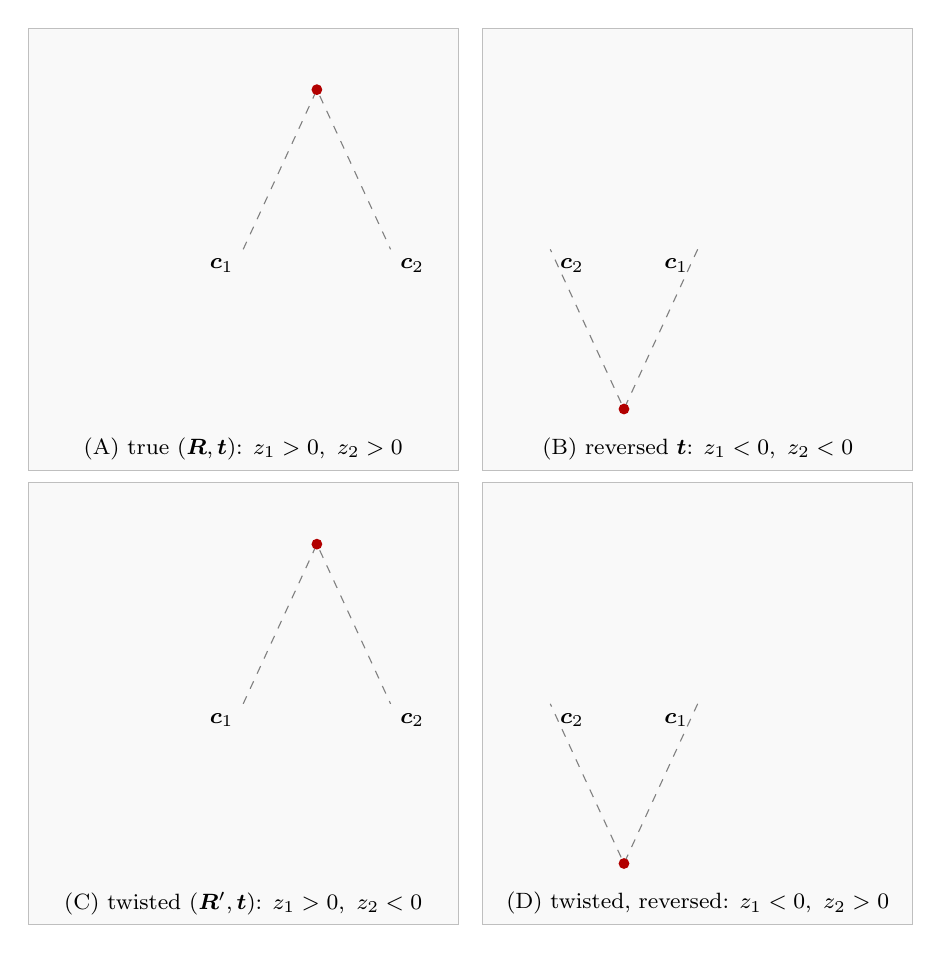
\begin{tikzpicture}[scale=0.78,every node/.style={font=\footnotesize}]
\foreach \name/\sx/\sy/\xc/\rot/\ptx/\pty/\lab in {
 A/0/0/2.4/0/1.2/2.6/{(A) true $(\bm R,\bm t)$: $z_1>0,\ z_2>0$},
 B/7.4/0/-2.4/0/-1.2/-2.6/{(B) reversed $\bm t$: $z_1<0,\ z_2<0$},
 C/0/-7.4/2.4/180/1.2/2.6/{(C) twisted $(\bm R',\bm t)$: $z_1>0,\ z_2<0$},
 D/7.4/-7.4/-2.4/180/-1.2/-2.6/{(D) twisted, reversed: $z_1<0,\ z_2>0$}}{
 \begin{scope}[shift={(\sx,\sy)}]
 \draw[gray!50,fill=gray!5] (-3.5,-3.6) rectangle (3.5,3.6);
 \draw[dashed,gray] (0,0)--(\ptx,\pty)--(\xc,0);
 \camdraw{0}{0}{0}
 \camdraw{\xc}{0}{\rot}
 \node[below left] at (0,0) {$\bm c_1$}; \node[below right] at (\xc,0) {$\bm c_2$};
 \fill[red!70!black] (\ptx,\pty) circle (2.5pt);
 \node at (0,-3.25) {\lab};
 \end{scope}}
\end{tikzpicture}
\caption{Schematic of the four candidate poses (after slide 27; in 2D, cameras drawn as triangles with an arrow along the viewing direction, red dot: reconstructed point, dashed: reconstructed rays). Only panel A has the point in front of both cameras.}
\label{fig:four}
\end{figure}

\begin{intuition}
The point is the same in all four panels; what changes is where the two cameras ``look''. If I flip the baseline, I must also look in the opposite direction to see the same image, so the point appears behind me. If I twist camera 2 around the baseline, camera 2 now looks away from the scene: the point is behind it but still in front of camera 1.
\end{intuition}

\subsection{Disambiguation by Cheirality \slr{28}}
\emph{Cheirality}: a reconstructed point must lie in front of both cameras. For each correspondence and each candidate $(\bm R_k,\bm t_k)$, the depths $z_1,z_2$ along the two rays follow from $\bm x_2=\bm R\bm x_1+\bm t$ with $\bm x_i=z_i\xt_i$:
\[
z_2\xt_2=z_1\bm R_k\xt_1+\bm t_k\iff\bigl[-\bm R_k\xt_1\ \ \xt_2\bigr]\begin{pmatrix}z_1\\z_2\end{pmatrix}=\bm t_k .
\]
Three equations, two unknowns: solve by least squares.

\begin{algorithm}{Pose from the essential matrix}{cheir}
\begin{enumerate}[nosep]
\item Decompose $\E$ into the four candidates (Thm.~\ref{thm:decomp}).
\item For each candidate and each correspondence solve the least-squares system above.
\item Keep the candidate with the most correspondences with $z_1>0$ and $z_2>0$. Count over \emph{all} points: noise and points near infinity can flip individual signs.
\end{enumerate}
Result: $[\bm R|\bm t]$, metric up to one global scale, fixed here by the convention $\norm{\bm t}=1$; later by the gauge of bundle adjustment (5.4) or by a normalization (5.5).
In OpenCV: \texttt{findEssentialMat} (5-point solver inside RANSAC), then \texttt{recoverPose} (decomposition and this test).
\end{algorithm}

\begin{example}{Cheirality in numbers}{cheirnum}
Use the rectified example: $u_1=0.1$, $u_2=0.3$, $\bm R=\bm I$. For $\bm t_k=(1,0,0)\tr$ the system
$\bigl[-\xt_1\ \xt_2\bigr](z_1,z_2)\tr=\bm t_k$ with $\xt_1=(0.1,v,1)\tr$, $\xt_2=(0.3,v,1)\tr$ reads $-0.1z_1+0.3z_2=1,\ -vz_1+vz_2=0,\ -z_1+z_2=0$, so $z_1=z_2=z$ and $0.2z=1$, $z=5>0$: accepted.
For $\bm t_k=(-1,0,0)\tr$ we get $0.2z=-1$, $z=-5<0$: the point would be behind both cameras: rejected.
\end{example}

\subsection{Estimating the Epipolar Geometry with Unknown Intrinsics \slr{29--30}}
If the calibration is unknown, we cannot use the local ray directions $\xt_i=\bm K_i^{-1}\xb_i$ and only know the pixel coordinates $\xb_i$.

\begin{definition}{Fundamental matrix}{fund}
Substituting $\xt_i=\bm K_i^{-1}\xb_i$ in the epipolar constraint gives
\[
\xt_2\tr\E\xt_1=\xb_2\tr\underbrace{\bm K_2^{-\mathsf T}\E\bm K_1^{-1}}_{\Fm}\xb_1=0 .
\]
$\Fm$ is the \emph{fundamental matrix}. Like $\E$ it is (without noise) of rank two and the epipoles can be recovered in the same way (as null vectors). The epipolar line of $\xb_1$ in image 2 is $\tilde{\bm l}_2=\Fm\xb_1$.
\end{definition}

The intrinsic parameters cannot be directly determined from $\Fm$ alone (a learned model that estimates the field of view directly from the images appears in 5.5).

\begin{intuition}
$\Fm$ is just $\E$ ``dressed'' in the unknown camera matrices: the same geometry, but expressed in pixels. It has 7 degrees of freedom (rank 2 and defined up to scale, $9-1-1$) instead of 5, because two extra parameters are not tied to a rigid motion. It is enough to draw epipolar lines and reject outliers, but you need $\bm K_i$ to convert it into a metric pose.
\end{intuition}

\imgph[4.0cm]{30}{Epipolar lines for two real images based on the estimated epipolar geometry; corresponding points lie on the corresponding epipolar lines.}

\subsection{Triangulation \slr{31--35}}
\paragraph{Problem (slide 32).} Given the camera intrinsics and extrinsics, how can we recover 3D geometry? With noisy 2D observations $\xb_1,\xb_2$ the two rays might not intersect; we want the 3D point $\bm x$ that is, in some sense, closest to the two rays (Fig.~\ref{fig:tri}).

\begin{figure}[H]
\centering
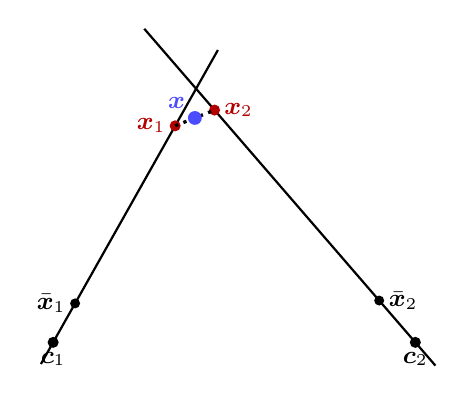
\begin{tikzpicture}[scale=1.0,every node/.style={font=\small}]
\coordinate (C1) at (0,0); \coordinate (C2) at (4.6,0);
\coordinate (P1) at (1.55,2.75); \coordinate (P2) at (2.05,2.95);
\draw[thick] ($(C1)!-0.1!(P1)$)--($(C1)!1.35!(P1)$);
\draw[thick] ($(C2)!-0.1!(P2)$)--($(C2)!1.35!(P2)$);
\fill (C1) circle (2pt) node[below]{$\bm c_1$}; \fill (C2) circle (2pt) node[below]{$\bm c_2$};
\fill[red!70!black] (P1) circle (2pt) node[left]{$\bm x_1$};
\fill[red!70!black] (P2) circle (2pt) node[right]{$\bm x_2$};
\draw[dotted,very thick] (P1)--(P2);
\fill[blue!70] ($(P1)!0.5!(P2)$) circle (2.5pt) node[above left,blue!70]{$\bm x$};
\fill ($(C1)!0.18!(P1)$) circle (1.8pt) node[left]{$\xb_1$};
\fill ($(C2)!0.18!(P2)$) circle (1.8pt) node[right]{$\xb_2$};
\end{tikzpicture}
\caption{Two noisy rays do not intersect; $\bm x_1,\bm x_2$ are their closest points and $\bm x$ their midpoint (slide 32).}\label{fig:tri}
\end{figure}

\begin{proposition}{Midpoint triangulation}{midpoint}
Let the rays be $\bm c_i+s_i\bm d_i$ ($\norm{\bm d_i}=1$) and $\bm b=\bm c_2-\bm c_1$. The closest points have parameters solving
\[
\begin{pmatrix}1&-\bm d_1\tr\bm d_2\\ \bm d_1\tr\bm d_2&-1\end{pmatrix}\begin{pmatrix}s_1\\s_2\end{pmatrix}=\begin{pmatrix}\bm d_1\tr\bm b\\ \bm d_2\tr\bm b\end{pmatrix},
\]
and the midpoint $\bm x=\tfrac12(\bm x_1+\bm x_2)$ minimizes the sum of squared distances to the two rays. The system degenerates exactly when $\bm d_1\parallel\bm d_2$.
\end{proposition}
\begin{proof}
Minimize $\norm{\bm c_1+s_1\bm d_1-\bm c_2-s_2\bm d_2}^2$. Setting the derivatives in $s_1,s_2$ to zero gives $\bm d_1\tr(s_1\bm d_1-s_2\bm d_2-\bm b)=0$ and $\bm d_2\tr(s_1\bm d_1-s_2\bm d_2-\bm b)=0$, which is the stated system. Its determinant is $-1+(\bm d_1\tr\bm d_2)^2=-\sin^2\gamma$, where $\gamma$ is the angle between the rays: zero iff the rays are parallel.
\end{proof}

\begin{intuition}
Two rays in 3D generically miss each other by a small gap; the segment joining their closest points is perpendicular to both. Taking its midpoint is the natural compromise. The determinant $\sin^2\gamma$ already hints at the next topic: when the rays are nearly parallel the problem becomes ill-conditioned.
\end{intuition}

\paragraph{Linear triangulation (DLT, slide 33).}
Let $\tilde{\bm x}^s_i=\tilde{\bm P}_i\tilde{\bm x}^w$ denote the projection of a 3D world point onto the image of the $i$-th camera. Both sides are homogeneous: they have the same direction but may differ in magnitude, so we consider the cross product $\bar{\bm x}^s_i\times\tilde{\bm P}_i\tilde{\bm x}^w=0$. With $\tilde{\bm p}_{ik}\tr$ the $k$-th row of $\tilde{\bm P}_i$ this gives
\[
\underbrace{\begin{pmatrix}x^s_i\,\tilde{\bm p}_{i3}\tr-\tilde{\bm p}_{i1}\tr\\ y^s_i\,\tilde{\bm p}_{i3}\tr-\tilde{\bm p}_{i2}\tr\end{pmatrix}}_{\bm A_i}\tilde{\bm x}^w=0 .
\]
Stacking $N\ge2$ observations yields $\bm A\tilde{\bm x}^w=0$. As $\tilde{\bm x}^w$ is homogeneous this is a constrained least-squares problem; the solution is the right singular vector of $\bm A$ with the smallest singular value (the Direct Linear Transformation, as for homography estimation in lecture 01).

\begin{intuition}
Each view contributes two independent linear equations (the third row of the cross product is a combination of the other two), and the unknown 3D point has 3 degrees of freedom, so two views already give $4\ge3$ equations. A single image of a point removes two degrees of freedom (it constrains the point to a line); the second one removes the rest and adds one redundant equation to absorb noise.
\end{intuition}

\paragraph{Reprojection error minimization (slide 34).} While DLT often works well, it is not invariant to projective transformations. The gold standard is to minimize the reprojection error numerically,
\[
\bar{\bm x}^*_w=\argmin_{\bar{\bm x}_w}\sum_{i=1}^N\norm{\bar{\bm x}^s_i(\bar{\bm x}_w)-\bar{\bm x}^o_i}_2^2,
\]
with observations $\bar{\bm x}^o_i$. This allows taking measurement noise appropriately into account. For two views the minimum can also be obtained in closed form as the solution of a sixth degree polynomial (Hartley and Zisserman, Section 12.5).

\paragraph{Triangulation uncertainty (slide 35).} Triangulation works differently well depending on the relative camera pose: uncertainty (shaded region) increases as the rays become more parallel. There is a \textbf{trade-off}: feature matching is easier for nearby views, but triangulation is harder. (A learned prior can also reconstruct views with little or no overlap, see 5.5.)

\begin{figure}[H]
\centering
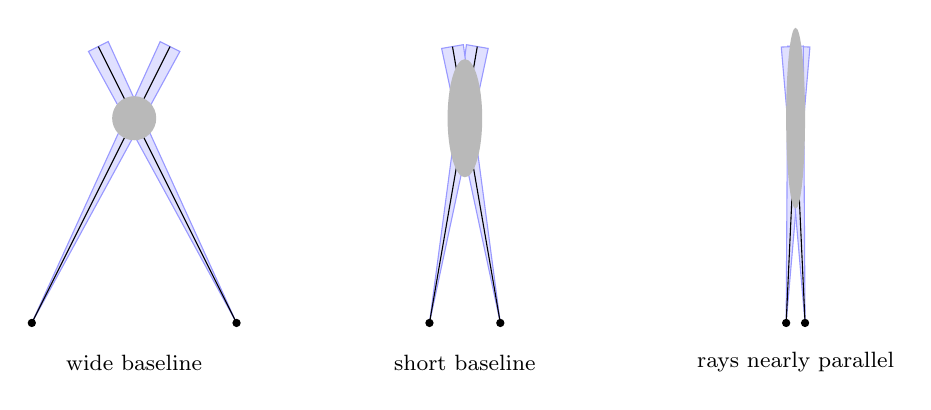
\begin{tikzpicture}[every node/.style={font=\footnotesize},
 cone/.style={fill=blue!12,draw=blue!40,thin}]
\foreach \cx/\cy/\ax/\ay/\bx/\by/\ex/\ey in {
  0/0/-1.3/0/1.3/0/0.28/0.28,
  4.2/0/-0.45/0/0.45/0/0.22/0.75,
  8.4/0/-0.12/0.0/0.12/0.0/0.12/1.15}{
 \begin{scope}[shift={(\cx,\cy)}]
 \coordinate (P) at (0,2.6); \coordinate (A) at (\ax,0); \coordinate (B) at (\bx,0);
 \foreach \C in {A,B}{
   \coordinate (Q) at ($(\C)!1.35!(P)$);
   \draw[cone] (\C)--($(Q)!0.14cm!90:(\C)$)--($(Q)!0.14cm!-90:(\C)$)--cycle;}
 \draw (A)--($(A)!1.35!(P)$) (B)--($(B)!1.35!(P)$);
 \fill[gray!55] (P) ellipse (\ex cm and \ey cm);
 \foreach \C in {A,B}{\fill (\C) circle(1.5pt);}
 \end{scope}}
\node at (0,-0.5) {wide baseline};\node at (4.2,-0.5) {short baseline};\node at (8.4,-0.5) {rays nearly parallel};
\end{tikzpicture}
\caption{Schematic of triangulation uncertainty (after slide 35): the grey region is where the two noisy rays are consistent with the observations. It grows as the rays become parallel. The ellipses are drawn by hand, not computed.}
\end{figure}

\begin{figure}[H]
\centering
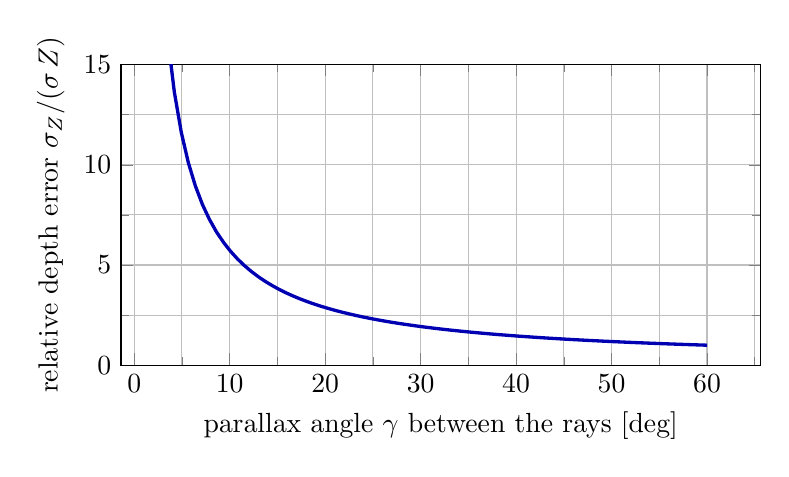
\begin{tikzpicture}
\begin{axis}[width=0.8\linewidth,height=5.4cm,xlabel={parallax angle $\gamma$ between the rays [deg]},
 ylabel={relative depth error $\sigma_Z/(\sigma\,Z)$},domain=2:60,samples=80,ymax=15,ymin=0,
 grid=both,minor tick num=1]
\addplot[very thick,blue!70!black] {1/(2*sin(x/2))};
\end{axis}
\end{tikzpicture}
\caption{Original illustration of the trade-off. For a point at distance $Z$ seen under angular noise $\sigma$ per ray, the depth error is, to first order, $\sigma_Z\approx\sigma Z/(2\sin(\gamma/2))\approx\sigma Z/\gamma$ (small $\gamma$). Below about $5^\circ$ the error explodes; above about $30^\circ$ it is flat, but matching becomes hard.}
\end{figure}

\begin{intuition}
Hold a finger at arm's length and look with one eye at a time: it jumps against the background. Do the same with a mountain: nothing moves. The jump is the parallax. Parallax is the signal that triangulation measures; if it is tiny, noise swamps it. Meanwhile large viewpoint changes make appearance very different, so matching fails. SfM pipelines therefore choose their image pairs carefully ('enough baseline for triangulation', slide 48).
\end{intuition}
%%%%%%%%%%%%%%%%%%%%%%%%%%%%%%%%%%%%%%%%%%%%%%%%%%%%%%%%%%%%%%%%%%%%%%
\section{Bundle Adjustment \slr{36--54}}

\subsection{Bundle Adjustment \slr{37--39}}
\imgph[3.8cm]{37}{Photo collection of Notre-Dame (left) and the resulting sparse reconstruction with camera frusta (right) (Snavely, Seitz and Szeliski, SIGGRAPH 2006).}

\textbf{Goal:} optimize the reprojection errors (distance between an observed feature and the projected 3D point in the image plane) with respect to the camera parameters and the 3D point cloud.

\begin{definition}{Bundle adjustment}{ba}
Let $\mathcal T=\{\bm T_i\}$ with $\bm T_i\in\SE$ ($i=1..N$) denote the camera poses; the calibrations $\bm K_i$ are known and fixed. Let $\mathcal X_w=\{\bm x^w_p\}$, $\bm x^w_p\in\R^3$ ($p=1..P$) be the 3D points in world coordinates and $\mathcal X_s=\{\bm x^s_{ip}\}$, $\bm x^s_{ip}\in\R^2$ the image observations in all cameras. Bundle adjustment minimizes the reprojection error of all observations:
\[
\mathcal T^*,\mathcal X_w^*=\argmin_{\mathcal T,\mathcal X_w}\sum_{i=1}^N\sum_{p=1}^P w_{ip}\,\bigl\lVert\bm x^s_{ip}-\pi_i(\bm x^w_p)\bigr\rVert_2^2,
\]
where $w_{ip}$ indicates whether point $p$ is observed in image $i$ and $\pi_i(\bm x^w_p)$ is the projection of the 3D world point into camera $i$ with its pose $\bm T_i=[\bm R_i|\bm t_i]$ and calibration $\bm K_i$:
\[
\pi_i(\bm x^w_p)=\begin{pmatrix}\tilde x^s_{ip}/\tilde w^s_{ip}\\ \tilde y^s_{ip}/\tilde w^s_{ip}\end{pmatrix},\qquad \tilde{\bm x}^s_{ip}=\bm K_i(\bm R_i\bm x^w_p+\bm t_i).
\]
\end{definition}

\begin{figure}[H]
\centering
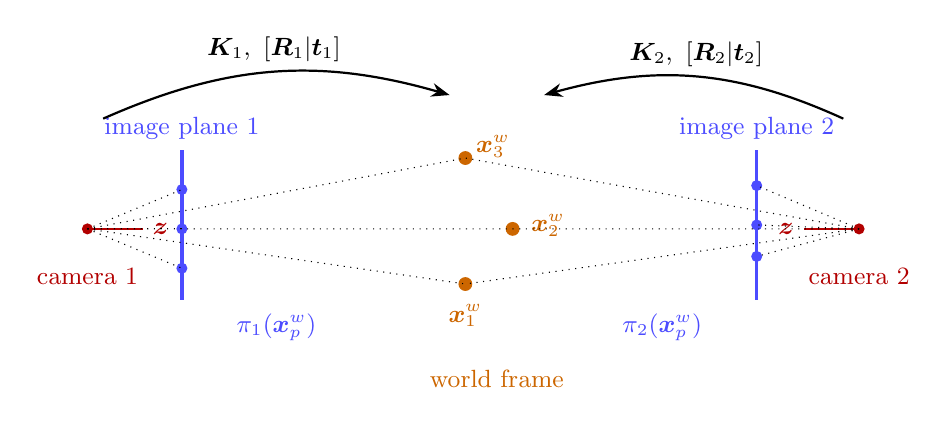
\begin{tikzpicture}[every node/.style={font=\small},scale=1.0]
% world points
\foreach \n/\x/\y in {1/0.2/-0.2,2/0.8/0.5,3/0.2/1.4}{\fill[orange!80!black] (\x,\y) circle (2.5pt);}
\node[orange!80!black] at (0.2,-0.6) {$\bm x^w_1$}; \node[orange!80!black] at (1.25,0.55) {$\bm x^w_2$}; \node[orange!80!black] at (0.55,1.55) {$\bm x^w_3$};
\node[orange!80!black] at (0.6,-1.4) {world frame};
% camera 1
\coordinate (c1) at (-4.6,0.5);
\draw[red!70!black,thick] (c1) -- ++(0.7,0) node[right]{$\bm z$}; \fill[red!70!black] (c1) circle (2pt);
\node[red!70!black] at (-4.6,-0.1) {camera 1};
\draw[blue!70,very thick] (-3.4,-0.4)--(-3.4,1.5) node[above]{image plane 1};
\foreach \y in {0.0,0.5,1.0}{\fill[blue!70] (-3.4,\y) circle (2pt); \draw[dotted] (c1)--(-3.4,\y);}
% camera 2
\coordinate (c2) at (5.2,0.5);
\draw[red!70!black,thick] (c2) -- ++(-0.7,0) node[left]{$\bm z$}; \fill[red!70!black] (c2) circle (2pt);
\node[red!70!black] at (5.2,-0.1) {camera 2};
\draw[blue!70,very thick] (3.9,-0.4)--(3.9,1.5) node[above]{image plane 2};
\foreach \y in {0.15,0.55,1.05}{\fill[blue!70] (3.9,\y) circle (2pt); \draw[dotted] (c2)--(3.9,\y);}
\draw[dotted] (c1)--(0.2,-0.2) (c1)--(0.8,0.5) (c1)--(0.2,1.4);
\draw[dotted] (c2)--(0.2,-0.2) (c2)--(0.8,0.5) (c2)--(0.2,1.4);
\draw[-{Stealth},thick] (-4.4,1.9) to[bend left=20] node[above]{$\bm K_1,\ [\bm R_1|\bm t_1]$} (0.0,2.2);
\draw[-{Stealth},thick] (5.0,1.9) to[bend right=20] node[above]{$\bm K_2,\ [\bm R_2|\bm t_2]$} (1.2,2.2);
\node[blue!70] at (-2.2,-0.75) {$\pi_1(\bm x^w_p)$}; \node[blue!70] at (2.7,-0.75) {$\pi_2(\bm x^w_p)$};
\end{tikzpicture}
\caption{The bundle adjustment setup (slide 39): the 3D points are projected into both cameras by $\pi_i$. With the $\bm K_i$ fixed, bundle adjustment optimizes the poses $\mathcal T$ and the points $\mathcal X_w$ jointly.}
\end{figure}

\begin{intuition}
Imagine each 3D point and each camera attached to the others by elastic bands: every observation is a band pulling the \emph{predicted} pixel towards the \emph{measured} pixel. The name ``bundle'' refers to the bundles of light rays between each camera center and its points. Adjusting them all at once (poses and points) finds the configuration where the total tension (squared reprojection error) is lowest. This is the maximum-likelihood estimate under independent isotropic Gaussian pixel noise.
\end{intuition}

\subsection{Challenges of Bundle Adjustment \slr{40}}
\begin{itemize}
\item \textbf{Initialization.} The energy landscape is highly non-convex: a good initialization is crucial to avoid bad local minima. As initializing all 3D points and cameras jointly is difficult (occlusion, viewpoint, matching outliers), \emph{incremental} bundle adjustment starts from a carefully selected two-view reconstruction and iteratively adds new images/cameras.
\item \textbf{Optimization.} With millions of features and thousands of cameras, large-scale bundle adjustment is computationally demanding (cubic complexity in the number of unknowns). Luckily the problem is \emph{sparse} (not every 3D point is observed in every camera), and efficient sparse implementations (e.g.\ g2o) can be exploited.
\item Here the calibrations $\bm K_i$ are fixed; bundle adjustment can also estimate one $\bm K_i$ per camera.
\item Predicting cameras and points with a network removes the incremental initialization (5.5).
\end{itemize}

\subsection{Bundle Adjustment as Nonlinear Least Squares \slr{41}}
Collect the unknowns in $\mathcal S=(\bm T_1,\dots,\bm T_N,\bm x^w_1,\dots,\bm x^w_P)$ with $\bm T_i=\begin{psmallmatrix}\bm R_i&\bm t_i\\\bm 0\tr&1\end{psmallmatrix}\in\SE$ and $\bm x^w_p\in\R^3$. Each residual compares the observation with the projection of the point, moved into camera $i$ by its pose:
\[
E(\mathcal S)=\sum_{i,p}w_{ip}\norm{\bm r_{ip}}_2^2,\qquad \bm r_{ip}=\bm x^s_{ip}-\pi\bigl(\bm K_i(\bm R_i\bm x^w_p+\bm t_i)\bigr),
\]
with the perspective division $\pi(\tilde x,\tilde y,\tilde w)=(\tilde x/\tilde w,\tilde y/\tilde w)$. Stacking all residuals into $\bm r(\mathcal S)$ gives $E(\mathcal S)=\norm{\bm r(\mathcal S)}_2^2$.
\begin{itemize}
\item $\pi_i$ contains a rotation and a perspective division: there is no closed form, and the minimization iterates from an initialization.
\item The poses do not form a vector space, so each iteration must update them on $\SE$.
\item $E$ does not change under a global rotation, translation and scale of all poses and points: these 7 degrees of freedom are fixed by holding one pose and one distance.
\end{itemize}

\begin{proposition}{Gauge freedom}{gauge}
Let $(\bm R_i,\bm t_i,\bm x^w_p)$ be any solution. For any rotation $\bm Q$, translation $\bm a$ and scale $\alpha>0$, define
$\bm x'^w_p=\alpha\bm Q\bm x^w_p+\bm a$, $\ \bm R'_i=\bm R_i\bm Q\tr$, $\ \bm t'_i=\alpha\bm t_i-\bm R_i\bm Q\tr\bm a$.
Then every projection, and hence $E$, is unchanged. Consequently $E$ is constant along a 7-dimensional family of solutions (the Hessian has a 7-dimensional null space).
\end{proposition}
\begin{proof}
$\bm R'_i\bm x'^w_p+\bm t'_i=\alpha\bm R_i\bm x^w_p+\bm R_i\bm Q\tr\bm a+\alpha\bm t_i-\bm R_i\bm Q\tr\bm a=\alpha(\bm R_i\bm x^w_p+\bm t_i)$,
so each camera-frame point is only multiplied by $\alpha$. Since a pixel is a ratio of coordinates, $\pi_i$ is invariant to scaling its argument, and all residuals are unchanged. The family has $3+3+1=7$ parameters.
\end{proof}

\begin{intuition}
The images do not know where the world origin is, which way is ``north'', or whether the scene is a toy or a real building (the scale ambiguity of Section 5.3). Fixing \emph{one pose} ($6$ dof: $\bm T_1=\bm I$) plus \emph{one distance} (1 dof: e.g.\ $\norm{\bm t_2}=1$) removes the 7 free directions; this is precisely the ``gauge'' chosen in the initialization of incremental SfM (slide 48).
\end{intuition}

\subsection{Updates in the Tangent Space \slr{42}}
A pose cannot be updated by addition: $\bm T_i+\Delta\bm T$ is in general not a rigid transformation, since $\bm R\tr\bm R=\bm I$ breaks, and its 12 entries carry only 6 degrees of freedom. The update is instead a 6-vector in the Lie algebra $\se\cong\R^6$, the tangent space of $\SE$, mapped onto the group by the exponential map. Points live in $\R^3$ and are added:
\[
\bm T_i\leftarrow\mathrm{Exp}(\Delta\bm\xi_i)\,\bm T_i,\qquad \bm x^w_p\leftarrow\bm x^w_p+\Delta\bm x_p,\qquad
\mathrm{Exp}(\Delta\bm\xi)=\exp\begin{pmatrix}\sk{\Delta\bm\omega}&\Delta\bm\rho\\\bm 0\tr&0\end{pmatrix},\ \ \Delta\bm\xi=(\Delta\bm\rho,\Delta\bm\omega),
\]
where $\Delta\bm\omega$ is an axis-angle rotation, $\Delta\bm\rho$ the translational part and $\exp$ the matrix exponential. The update is \emph{minimal and unconstrained}: 6 numbers per pose, and every update stays in $\SE$.

\begin{figure}[H]
\centering
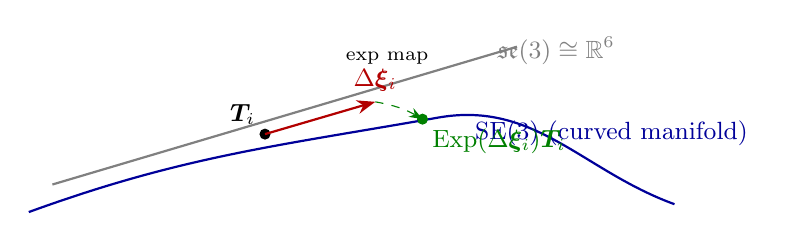
\begin{tikzpicture}[every node/.style={font=\small}]
\draw[thick,blue!60!black] (0,0) to[out=20,in=190] (5.2,1.2) to[out=10,in=160] (8.2,0.1);
\node[blue!60!black] at (7.4,1.0) {$\SE$ (curved manifold)};
\coordinate (T) at (3.0,0.99);
\fill (T) circle (2pt) node[above left]{$\bm T_i$};
\draw[thick,gray] (0.3,0.35)--(6.2,2.1) ; 
\node[gray] at (6.7,2.05) {$\se\cong\R^6$};
\draw[-{Stealth},thick,red!70!black] (T)--(4.4,1.4) node[above]{$\Delta\bm\xi_i$};
\fill[green!50!black] (5.0,1.18) circle (2pt) node[below right]{$\mathrm{Exp}(\Delta\bm\xi_i)\bm T_i$};
\draw[-{Stealth},dashed,green!50!black] (4.4,1.4) to[bend left=10] (5.0,1.18);
\node at (4.55,1.95) {\scriptsize exp map};
\end{tikzpicture}
\caption{Local update on a curved space: take a step $\Delta\bm\xi_i$ in the flat tangent space, then map it back onto the group with the exponential map (schematic).}
\end{figure}

\begin{beyond}
For $\theta=\norm{\Delta\bm\omega}$ the exponential has a closed form (Rodrigues): $\exp\sk{\Delta\bm\omega}=\bm I+\frac{\sin\theta}{\theta}\sk{\Delta\bm\omega}+\frac{1-\cos\theta}{\theta^2}\sk{\Delta\bm\omega}^2$, and $\mathrm{Exp}(\Delta\bm\xi)=\begin{psmallmatrix}\exp\sk{\Delta\bm\omega}&\bm V\Delta\bm\rho\\\bm0\tr&1\end{psmallmatrix}$ with $\bm V=\bm I+\frac{1-\cos\theta}{\theta^2}\sk{\Delta\bm\omega}+\frac{\theta-\sin\theta}{\theta^3}\sk{\Delta\bm\omega}^2$.
\end{beyond}

\begin{intuition}
Think of walking on the surface of the Earth: you plan a step on a flat map (the tangent plane) and then ``wrap'' it back onto the sphere. If you added numbers straight into the 12 matrix entries you would step \emph{off} the surface (the matrix stops being a rotation).
\end{intuition}

\subsection{The Gauss--Newton Algorithm \slr{43}}
Each residual depends on one pose and one point. Around the current estimate it is linearized in their increments:
\[
\bm r_{ip}\bigl(\mathrm{Exp}(\Delta\bm\xi_i)\bm T_i,\ \bm x^w_p+\Delta\bm x_p\bigr)\approx\bm r_{ip}+\bm J^{\xi}_{ip}\Delta\bm\xi_i+\bm J^x_{ip}\Delta\bm x_p .
\]

\begin{lemma}{Jacobians of the reprojection residual}{jac}
With $\bm x^c_{ip}=\bm R_i\bm x^w_p+\bm t_i$ and $\bm J_\pi\in\R^{2\times3}$ the Jacobian of the projection $\bm x^c\mapsto\pi(\bm K_i\bm x^c)$ (so $\bm J_\pi=\bigl(\partial\pi/\partial\tilde{\bm x}\bigr)\bm K_i$), both blocks at zero increment are
\[
\bm J^{\xi}_{ip}=-\bm J_\pi\bigl[\ \bm I\ \ \ -\sk{\bm x^c_{ip}}\ \bigr]\in\R^{2\times6},\qquad
\bm J^x_{ip}=-\bm J_\pi\bm R_i\in\R^{2\times3}.
\]
\end{lemma}
\begin{proof}
For a small $\Delta\bm\xi=(\Delta\bm\rho,\Delta\bm\omega)$, $\mathrm{Exp}(\Delta\bm\xi)\approx\bm I+\begin{psmallmatrix}\sk{\Delta\bm\omega}&\Delta\bm\rho\\\bm 0\tr&0\end{psmallmatrix}$, so the camera-frame point becomes
$\bm x^c+\Delta\bm\omega\times\bm x^c+\Delta\bm\rho=\bm x^c+\Delta\bm\rho-\sk{\bm x^c}\Delta\bm\omega$. The residual is $\bm x^s-\pi(\bm K\bm x^c)$, so by the chain rule $\partial\bm r/\partial\Delta\bm\xi=-\bm J_\pi[\bm I\ \ -\sk{\bm x^c}]$.
A change $\Delta\bm x$ of the world point changes $\bm x^c$ by $\bm R_i\Delta\bm x$, giving $-\bm J_\pi\bm R_i$.
\end{proof}

\begin{intuition}
The first block says: moving the camera by $\Delta\bm\rho$ is the same as moving the point by $\Delta\bm\rho$ in the camera frame, while rotating by $\Delta\bm\omega$ moves the point sideways by an amount proportional to its distance ($\Delta\bm\omega\times\bm x^c$): far points are sensitive to rotation, near points to translation. The leading minus sign comes from $\bm r=\text{observed}-\text{predicted}$.
\end{intuition}

With all increments stacked into $\Delta\bm s=(\Delta\bm\xi_1,\dots,\Delta\bm\xi_N,\Delta\bm x_1,\dots,\Delta\bm x_P)\in\R^{6N+3P}$, minimizing $\norm{\bm r+\bm J\Delta\bm s}_2^2$ gives the normal equations; the update is repeated until convergence:
\[
\bm H\Delta\bm s=-\bm b,\quad \bm H=\bm J\tr\bm J,\quad\bm b=\bm J\tr\bm r,\qquad \bm T_i\leftarrow\mathrm{Exp}(\Delta\bm\xi_i)\bm T_i,\ \ \bm x^w_p\leftarrow\bm x^w_p+\Delta\bm x_p .
\]

\begin{algorithm}{Gauss--Newton for bundle adjustment}{gn}
\begin{enumerate}[nosep]
\item Start from an initialization $\mathcal S_0$ (e.g.\ two-view reconstruction).
\item Compute all residuals $\bm r_{ip}$ and Jacobians (Lemma~\ref{lem:jac}).
\item Build $\bm H=\bm J\tr\bm J$ and $\bm b=\bm J\tr\bm r$ and solve $\bm H\Delta\bm s=-\bm b$ (exploiting sparsity, next subsection).
\item Update poses on $\SE$ and points in $\R^3$; repeat steps 2--4 until $\norm{\Delta\bm s}$ or the decrease of $E$ is small.
\end{enumerate}
\end{algorithm}

\begin{beyond}
In practice, Levenberg--Marquardt is used: $(\bm H+\lambda\bm D)\Delta\bm s=-\bm b$ with a damping $\lambda$ that interpolates between Gauss--Newton ($\lambda\to0$, fast near the minimum) and gradient descent ($\lambda$ large, safe far away). Robust loss functions (Huber, Cauchy) are commonly applied to reduce the effect of outliers. COLMAP uses the solver Ceres (slide 51).
\end{beyond}

\subsection{The Schur Complement \slr{44}}
With the pose increments $\Delta\bm\xi\in\R^{6N}$ ordered before the point increments $\Delta\bm x\in\R^{3P}$, the normal equations read
\[
\begin{pmatrix}\bm H_{\xi\xi}&\bm H_{\xi x}\\\bm H_{x\xi}&\bm H_{xx}\end{pmatrix}\begin{pmatrix}\Delta\bm\xi\\\Delta\bm x\end{pmatrix}=-\begin{pmatrix}\bm b_\xi\\\bm b_x\end{pmatrix}.
\]
$\bm H_{xx}$ is block diagonal, one $3\times3$ block per point, so its inverse is cheap. Eliminating the points leaves a system in the $6N$ pose increments alone, and back substitution recovers the points.

\begin{theorem}{Schur complement reduction}{schur}
If $\bm H_{xx}$ is invertible, the pose increments solve
\[
\bigl(\bm H_{\xi\xi}-\bm H_{\xi x}\bm H_{xx}^{-1}\bm H_{x\xi}\bigr)\Delta\bm\xi=-\bigl(\bm b_\xi-\bm H_{\xi x}\bm H_{xx}^{-1}\bm b_x\bigr),
\qquad
\Delta\bm x=-\bm H_{xx}^{-1}\bigl(\bm b_x+\bm H_{x\xi}\Delta\bm\xi\bigr),
\]
and these give the same pose update as the full system.
\end{theorem}
\begin{proof}
The second block row reads $\bm H_{x\xi}\Delta\bm\xi+\bm H_{xx}\Delta\bm x=-\bm b_x$, which gives $\Delta\bm x$ as stated. Substituting it into the first block row,
$\bm H_{\xi\xi}\Delta\bm\xi-\bm H_{\xi x}\bm H_{xx}^{-1}(\bm b_x+\bm H_{x\xi}\Delta\bm\xi)=-\bm b_\xi$, and rearranging gives the reduced system.
\end{proof}

The matrix on the left, $\bm S=\bm H_{\xi\xi}-\bm H_{\xi x}\bm H_{xx}^{-1}\bm H_{x\xi}$, is the Schur complement of $\bm H_{xx}$ in $\bm H$. It yields the same pose update from $6N$ unknowns instead of $6N+3P$: thousands instead of millions. Each point is then updated independently.

\begin{figure}[H]
\centering
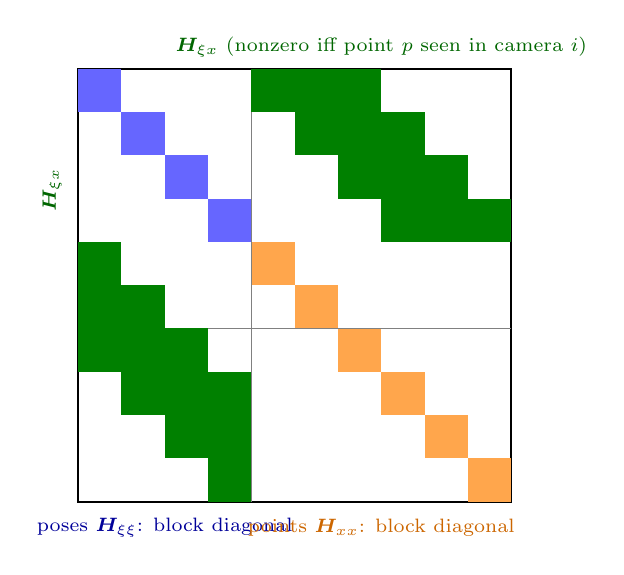
\begin{tikzpicture}[scale=0.55,every node/.style={font=\scriptsize}]
% matrix of size (4 pose blocks)+(6 point blocks)
\def\s{1}
\draw[thick] (0,0) rectangle (10,10);
% pose diagonal blocks (top-left): 4 blocks of size 1
\foreach \i in {0,...,3}{\fill[blue!60] (\i,9-\i) rectangle (\i+1,10-\i);}
% point diagonal blocks (bottom-right): 6 blocks
\foreach \p in {0,...,5}{\fill[orange!70] (4+\p,5-\p-0) rectangle (5+\p,6-\p-0);}
\draw[gray,thin] (4,0) -- (4,10); \draw[gray,thin] (0,4) -- (10,4);
% observations: (camera, point)
\foreach \c/\p in {0/0,0/1,0/2,1/1,1/2,1/3,2/2,2/3,2/4,3/3,3/4,3/5}{
 \fill[green!50!black] (4+\p,9-\c) rectangle (5+\p,10-\c);
 \fill[green!50!black] (\c,5-\p) rectangle (\c+1,6-\p);}
\node[blue!60!black] at (2,-0.6) {poses $\bm H_{\xi\xi}$: block diagonal};
\node[orange!80!black] at (7,-0.6) {points $\bm H_{xx}$: block diagonal};
\node[green!40!black,rotate=90] at (-0.6,7.2) {$\bm H_{\xi x}$};
\node[green!40!black] at (7,10.5) {$\bm H_{\xi x}$ (nonzero iff point $p$ seen in camera $i$)};
\end{tikzpicture}
\caption{Arrowhead sparsity of the BA Hessian for $N=4$ cameras and $P=6$ points (original illustration). Cameras and points interact only if they share an observation. Eliminating the points (orange) leaves a small $4\times4$-block reduced camera system.}
\end{figure}

\begin{example}{Why the Schur complement matters}{schurnum}
Take $N=100$ cameras and $P=100{,}000$ points (a modest dataset). The full system has $6N+3P=300{,}600$ unknowns, a dense solve would cost $\sim(3\cdot10^5)^3\approx2.7\cdot10^{16}$ operations.
The reduced system has $6N=600$ unknowns, costing $\sim600^3\approx2.2\cdot10^8$ operations; the $10^5$ small $3\times3$ inversions are trivial.
That is a factor of about $10^8$.
\end{example}

\begin{intuition}
The points never talk directly to each other, only through the cameras that see them. So we can ``integrate out'' each point (a tiny $3\times3$ problem), which replaces the point-to-camera coupling by an additional camera-to-camera coupling for every pair of cameras that share a point. After solving for the cameras, each point just reads the new camera positions and updates itself. (This is the standard trick behind \emph{reduced camera systems} in Triggs et al.\ 2000.)
\end{intuition}

\subsection{Incremental Structure-from-Motion \slr{45--51}}
The feature matching and reconstruction pipeline (COLMAP, Sch\"onberger and Frahm 2016) has two big stages (Fig.~\ref{fig:colmap}): \textbf{correspondence search} (find and match robust 2D features across images) and \textbf{incremental reconstruction} (start with two views and incrementally add cameras).

\begin{figure}[H]
\centering
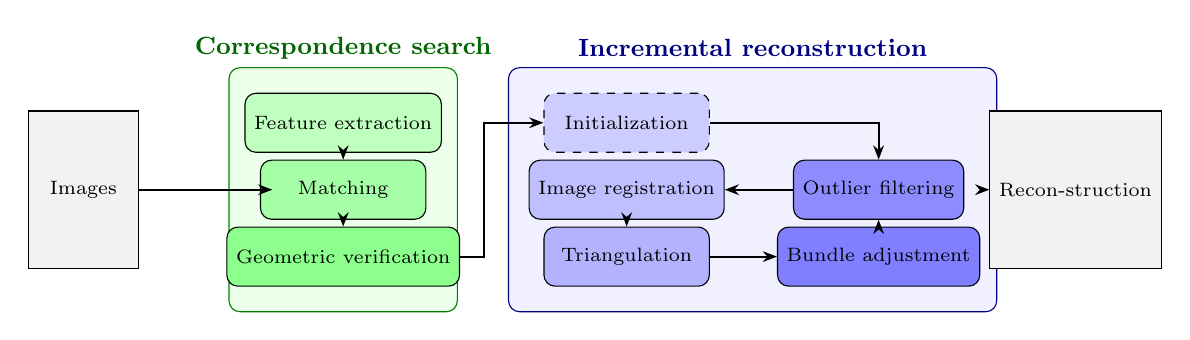
\begin{tikzpicture}[node distance=0.4cm,every node/.style={font=\scriptsize},
 b/.style={draw,rounded corners,minimum height=0.75cm,minimum width=2.1cm,align=center},
 arr/.style={-{Stealth[length=1.8mm]},thick}]
\node[draw,fill=gray!10,minimum width=1.4cm,minimum height=2cm,align=center] (img) at (0,0) {Images};
\begin{scope}[on background layer]
\node[draw=green!50!black,fill=green!8,rounded corners,minimum width=2.9cm,minimum height=3.1cm] at (3.3,0) {};
\node[draw=blue!50!black,fill=blue!6,rounded corners,minimum width=6.2cm,minimum height=3.1cm] at (8.5,0) {};
\end{scope}
\node[font=\small\bfseries,green!40!black] at (3.3,1.8) {Correspondence search};
\node[font=\small\bfseries,blue!50!black] at (8.5,1.8) {Incremental reconstruction};
\node[b,fill=green!25] (fe) at (3.3,0.85) {Feature extraction};
\node[b,fill=green!35] (ma) at (3.3,0) {Matching};
\node[b,fill=green!45] (gv) at (3.3,-0.85) {Geometric verification};
\node[b,fill=blue!20,dashed] (in) at (6.9,0.85) {Initialization};
\node[b,fill=blue!25] (ir) at (6.9,0) {Image registration};
\node[b,fill=blue!30] (tr) at (6.9,-0.85) {Triangulation};
\node[b,fill=blue!45] (of) at (10.1,0.0) {Outlier filtering};
\node[b,fill=blue!50] (ba) at (10.1,-0.85) {Bundle adjustment};
\node[draw,fill=gray!10,minimum width=1.7cm,minimum height=2cm,align=center] (rec) at (12.6,0) {Recon-struction};
\draw[arr](img)--(2.4,0);
\draw[arr](fe)--(ma);\draw[arr](ma)--(gv);
\draw[arr](gv.east)--++(0.3,0)|-(in.west);
\draw[arr](in.east)-|(of.north);
\draw[arr](of.west)--(ir.east);
\draw[arr](ir)--(tr);\draw[arr](tr)--(ba);\draw[arr](ba)--(of);
\draw[arr](11.4,0)--(rec.west);
\end{tikzpicture}
\caption{Incremental SfM pipeline of COLMAP (redrawn from slide 45). The registration--triangulation--filtering--bundle-adjustment loop runs once per added image.}
\label{fig:colmap}
\end{figure}

\paragraph{Feature extraction (slide 46).} Detect features (e.g.\ SIFT, SURF, BRISK) in all input images.
\imgph[3.4cm]{46}{Features detected on a photograph of a monument: boxes show location, scale and orientation of each feature (Sch\"onberger and Frahm, CVPR 2016).}

\paragraph{Feature matching and geometric verification (slide 47).} Find overlapping image pairs and the associated feature correspondences. Candidate matches are verified geometrically, i.e.\ they are kept only if they are consistent with an epipolar geometry or homography (RANSAC).
\imgph[3.8cm]{47}{Graph of images (nodes) connected when they overlap; example photos of the Trevi fountain at different scales and lighting (Sch\"onberger and Frahm, CVPR 2016).}

\paragraph{Initialization (slide 48).}
\begin{algorithm}{SfM initialization from two views}{init}
\begin{enumerate}[nosep]
\item Select \textbf{two views} with many correspondences $\xb_1\leftrightarrow\xb_2$ and enough baseline for triangulation.
\item Estimate $\E$ from $\xt_2\tr\E\xt_1=0$, with $\xt_i=\bm K_i^{-1}\xb_i$, by the 5-point solver inside RANSAC.
\item Decompose $\E$ into $[\bm R|\bm t]$ and keep the candidate that puts the points in front of both cameras (Alg.~\ref{alg:cheir}).
\item Fix the gauge: $\bm T_1=\bm I$ and $\bm T_2=[\bm R|\bm t]$ with $\norm{\bm t}=1$ (this removes the 7 gauge degrees of freedom, Prop.~\ref{prop:gauge}).
\item \textbf{Triangulate} the inliers to obtain the first points $\bm x^w_p$.
\end{enumerate}
\end{algorithm}

\paragraph{Image registration (slide 49).} Find a new image with correspondences to the current set and estimate its camera pose. Let $\mathcal X=\{\bar{\bm x}^s_i,\bar{\bm x}^w_i\}_{i=1}^N$ be a set of 3D-to-2D correspondences related by $\bar{\bm x}^s_i=\bm P\bar{\bm x}^w_i$. As the vectors are homogeneous, they have the same direction but differ in magnitude, so the equation can be expressed as $\bar{\bm x}^s_i\times\bm P\bar{\bm x}^w_i=0$. Using the Direct Linear Transform this is a linear equation in the entries of $\bm P$; the solution of the constrained system (fixing $\bm P$'s scale) is given by SVD.
Given that $\bm P=\bm K[\bm R|\bm t]$ and $\bm K$ is upper-triangular, both $\bm K$ and $\bm R$ can be obtained from the $3\times3$ front submatrix of $\bm P$ by standard RQ factorization. If $\bm K$ is known, we can even estimate $\bm P$ from only three points (P3P). In practice, RANSAC is used to remove outliers.

\begin{intuition}
Registration is the ``PnP'' problem: given a few points whose 3D position is already known from earlier triangulation, find where the new camera stands. $\bm P$ has 11 degrees of freedom (a $3\times4$ matrix up to scale) and every 3D--2D pair provides two independent equations, so DLT needs at least 6 points ($11/2=5.5$, rounded up). If $\bm K$ is known only 6 unknowns remain, and 3 points (6 equations) suffice, at the price of up to four solutions (P3P). Triangulation (known cameras $\to$ points) and registration (known points $\to$ camera) alternate: this is how the reconstruction ``crawls'' outwards.
\end{intuition}

\paragraph{Triangulation (slide 50).} Given the newly registered image, new correspondences can be triangulated. In COLMAP, a robust triangulation method handles outliers.

\paragraph{Bundle adjustment and outlier filtering (slide 51).} Minimize the reprojection error of all observations with respect to all poses and 3D points (Def.~\ref{def:ba}). Since incremental SfM only affects the model locally, COLMAP performs \emph{local} BA on the locally connected images, and \emph{global} BA only once in a while for efficiency. For the sparse large-scale optimization it uses Ceres. After each BA, observations with large reprojection errors and cameras with abnormal fields of view or large distortion coefficients are removed.

\begin{algorithm}{Incremental SfM (COLMAP-style)}{incsfm}
\begin{enumerate}[nosep]
\item Extract features in all images, match overlapping pairs, verify geometrically.
\item Initialize with a two-view reconstruction (Alg.~\ref{alg:init}).
\item \textbf{Repeat} until no image can be added: register the best new image (DLT/P3P inside RANSAC); triangulate new points; run local BA; filter outliers (large reprojection error, abnormal cameras); occasionally run global BA.
\end{enumerate}
\end{algorithm}

\begin{intuition}
Because the cost is highly non-convex, you ``grow a crystal'': start from a tiny well-conditioned seed (two views) and add only what is consistent with it, re-optimizing after each addition so errors never accumulate far from where the optimizer can fix them. The price: images are registered one at a time, so an early mistake propagates (a limit discussed in 5.5).
\end{intuition}

\subsection{Building Rome in a Day, COLMAP SfM and COLMAP MVS \slr{52--54}}
\begin{itemize}
\item \textbf{Building Rome in a Day} (Agarwal et al., ICCV 2009): first large-scale SfM from unstructured images (slide 52).
\item \textbf{COLMAP} significantly improves accuracy and robustness compared to prior work (slide 53).
\item COLMAP features a second \textbf{multi-view stereo} stage to obtain dense geometry (slide 54; Sch\"onberger et al., ECCV 2016). A feed-forward network predicts dense depth without known cameras (5.5), whereas MVS needs SfM first.
\end{itemize}
\imgph[3.6cm]{52}{Sparse point cloud and camera frusta of the Colosseum reconstructed from internet photos (Agarwal, Snavely, Simon, Seitz and Szeliski, ``Building Rome in a Day'', ICCV 2009).}
\imgph[3.6cm]{53}{COLMAP sparse reconstruction of a city scene; red marks the camera positions (Sch\"onberger and Frahm, CVPR 2016).}
\imgph[3.6cm]{54}{Dense COLMAP multi-view stereo reconstruction of a building (Sch\"onberger, Zheng, Frahm and Pollefeys, ECCV 2016).}
%%%%%%%%%%%%%%%%%%%%%%%%%%%%%%%%%%%%%%%%%%%%%%%%%%%%%%%%%%%%%%%%%%%%%%
\section{Feed-Forward Structure-from-Motion \slr{55--68}}

\subsection{Limits of Incremental Structure-from-Motion \slr{56}}
Looking back at Fig.~\ref{fig:colmap}:
\begin{itemize}
\item every box is a separately engineered stage, with its own thresholds and failure cases;
\item images are registered one at a time: a poor initial pair, outliers or drift propagate to every later image;
\item runtime grows to hours for large photo collections; few views, low overlap or little texture leave too few correspondences;
\item \textbf{Global SfM} estimates all cameras jointly without learning: rotation averaging, then camera positions, then one bundle adjustment. GLOMAP (Pan, Bar\'ath, Pollefeys and Sch\"onberger, ECCV 2024), a recent global pipeline, is on par with COLMAP in accuracy and orders of magnitude faster.
\end{itemize}

\begin{intuition}
Incremental SfM is like building a house brick by brick with one mason: reliable but slow, and a crooked first brick tilts the whole house. Global SfM hires many masons who work simultaneously and then reconcile. Feed-forward SfM, the topic of this section, replaces the masons by a single network that has seen millions of houses and sketches the whole building at once.
\end{intuition}

\subsection{From Learned Components to Learned Reconstruction \slr{57}}
\begin{table}[H]
\centering
\begin{tabular}{@{}llp{9.3cm}@{}}
\toprule
Year & Method & What is learned\\
\midrule
2018 & SuperPoint & keypoints and their descriptors, from one network (5.2)\\
2020 & SuperGlue & the matching of two keypoint sets, with a graph neural network\\
2021 & LoFTR & dense matches between two images, with a transformer and no detector\\
2024 & VGGSfM & a complete SfM pipeline, differentiable, trained end to end\\
2024 & DUSt3R, MASt3R & pointmaps from two images (lecture 04); more views need a global alignment\\
2025 & VGGT & cameras, depth, point maps and tracks for many views, in one forward pass\\
\bottomrule
\end{tabular}
\caption{Progressive replacement of the classical pipeline by learned components (slide 57).}
\end{table}

\begin{definition}{Pointmap}{pointmap}
For an $H\times W$ image $\bm I_a$, the pointmap $\hat{\bm X}^{a,1}\in\R^{H\times W\times3}$ stores \emph{one 3D point per pixel}, for both images $a\in\{1,2\}$, expressed in the frame of camera 1.
\end{definition}

\begin{figure}[H]
\centering
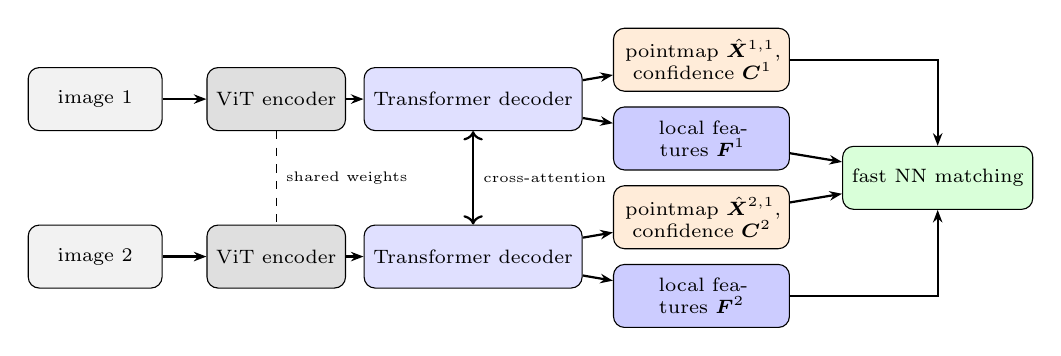
\begin{tikzpicture}[node distance=0.35cm,every node/.style={font=\scriptsize},
 b/.style={draw,rounded corners,minimum height=0.8cm,minimum width=1.7cm,align=center},
 arr/.style={-{Stealth[length=1.6mm]},thick}]
\node[b,fill=gray!10] (i1) at (0,1.0) {image 1};
\node[b,fill=gray!10] (i2) at (0,-1.0) {image 2};
\node[b,fill=gray!25] (e1) at (2.3,1.0) {ViT encoder};
\node[b,fill=gray!25] (e2) at (2.3,-1.0) {ViT encoder};
\draw[dashed] (e1)--(e2) node[midway,right,font=\tiny]{shared weights};
\node[b,fill=blue!12] (d1) at (4.8,1.0) {Transformer decoder};
\node[b,fill=blue!12] (d2) at (4.8,-1.0) {Transformer decoder};
\draw[<->,thick] (d1)--(d2) node[midway,right,font=\tiny]{cross-attention};
\node[b,fill=orange!15,text width=2cm] (p1) at (7.7,1.5) {pointmap $\hat{\bm X}^{1,1}$, confidence $\bm C^1$};
\node[b,fill=blue!20,text width=2cm] (f1) at (7.7,0.5) {local features $\bm F^1$};
\node[b,fill=orange!15,text width=2cm] (p2) at (7.7,-0.5) {pointmap $\hat{\bm X}^{2,1}$, confidence $\bm C^2$};
\node[b,fill=blue!20,text width=2cm] (f2) at (7.7,-1.5) {local features $\bm F^2$};
\node[b,fill=green!15] (m) at (10.7,0) {fast NN matching};
\draw[arr](i1)--(e1);\draw[arr](i2)--(e2);\draw[arr](e1)--(d1);\draw[arr](e2)--(d2);
\draw[arr](d1)--(p1);\draw[arr](d1)--(f1);\draw[arr](d2)--(p2);\draw[arr](d2)--(f2);
\draw[arr](p1)-|(m);\draw[arr](f1)--(m);\draw[arr](p2)--(m);\draw[arr](f2)-|(m);
\end{tikzpicture}
\caption{MASt3R-style two-view network (simplified from slide 57): tokens $\bm H^a$ from a ViT encoder are decoded with cross-attention into pointmaps with confidence (grey path) and local features (blue path), used for geometrical or feature-based matching.}
\end{figure}

\begin{intuition}
A pointmap is a depth map that already lives in a common world frame: once pixel $(u,v)$ of image 2 and pixel $(u',v')$ of image 1 carry (almost) the same 3D point, they are a correspondence \emph{by construction}. DUSt3R and MASt3R use this to skip the detect-describe-match-verify chain, but for more than two images they still need a post-hoc global alignment; VGGT removes that last step.
\end{intuition}

\subsection{Visual Geometry Grounded Transformer (VGGT) \slr{58}}
\begin{itemize}
\item \textbf{Input:} one to hundreds of images of a scene; the first image defines the world frame.
\item \textbf{Output,} in one forward pass of under a second: camera parameters, depth maps, point maps and point tracks for every image.
\item Without post-processing, it often outperforms methods that refine their output by geometric optimization.
\end{itemize}
\imgph[4.2cm]{58}{VGGT takes a set of images of a scene (left) and predicts, in one forward pass, camera poses, a dense point cloud, depth maps and point tracks (Wang et al., CVPR 2025).}

\subsection{Problem Definition \slr{59}}
\begin{definition}{VGGT as a function}{vggtdef}
VGGT is one network with learned weights $\theta$. It takes $N$ images $\bm I_1,\dots,\bm I_N$, each of $H\times W$ pixels, and predicts four outputs per image $i$ (the hat marks a prediction):
\[
f_\theta(\bm I_1,\dots,\bm I_N)=\bigl(\hat{\bm g}_i,\ \hat{\bm D}_i,\ \hat{\bm X}_i,\ \bm F_i\bigr)_{i=1}^N .
\]
\begin{itemize}[nosep]
\item \textbf{Camera} $\hat{\bm g}_i\in\R^9$: rotation quaternion $\hat{\bm q}_i\in\R^4$, translation $\hat{\bm t}_i\in\R^3$ and field of view $\hat{\bm\phi}_i=(\hat\phi_x,\hat\phi_y)$. They give the pose $\bm T_i$ and the calibration $\bm K_i$ with focal lengths $f_x=W/(2\tan(\phi_x/2))$, $f_y=H/(2\tan(\phi_y/2))$ and the principal point at the image center.
\item \textbf{Depth map} $\hat{\bm D}_i\in\R^{H\times W}$: the depth of every pixel.
\item \textbf{Point map} $\hat{\bm X}_i\in\R^{H\times W\times3}$: the 3D point of every pixel, in the frame of camera 1, which is the world frame.
\item \textbf{Feature map} $\bm F_i\in\R^{H\times W\times C}$: $C$ numbers per pixel, used to track points across the images.
\end{itemize}
\end{definition}
The outputs are redundant, since the cameras follow from the point maps (PnP), yet predicting all of them improves accuracy.

\begin{example}{From field of view to focal length}{fov}
For $W=518$ pixels and a predicted horizontal field of view $\phi_x=60^\circ$: $f_x=518/(2\tan30^\circ)=518/1.1547\approx449$ pixels. With the principal point at $(259,259)$ this fully specifies $\bm K$ (no calibration needed, in contrast to Section 5.1).
\end{example}

\begin{intuition}
Classical SfM needs $\bm K$ from calibration or self-calibration (and fails when it is wrong). VGGT simply \emph{guesses} the field of view from the image content as a human would (a wide-angle shot looks different from a telephoto one). Predicting the same geometry in several forms (cameras, depth, point maps) gives the network several consistent ``views'' of one underlying 3D structure to learn from.
\end{intuition}

\subsection{Architecture: Alternating Attention \slr{60}}
\begin{itemize}
\item \textbf{Image tokens,} as $\bm H^a$ in DUSt3R: a vision transformer (DINO) cuts each image $\bm I_i$ into patches and turns each patch into a token, a feature vector.
\item \textbf{Camera token:} a transformer returns one vector per input token. A $518\times518$ image gives $37\times37=1369$ patch tokens, hence 1369 outputs, one per patch, for the per-pixel maps. One extra learned token per image, the same for every image, yields one extra output: the camera head reads $\hat{\bm g}_i$ from it.
\item \textbf{Alternating attention,} $L=24$ times: \emph{global attention} among the tokens of all images (as the cross-attention of DUSt3R but for $N$ images), then \emph{frame attention} among the tokens of one image.
\item \textbf{Outputs:} the camera head turns each camera token into $\hat{\bm g}_i$; the DPT (Dense Prediction Transformer) head turns the image tokens into $\hat{\bm D}_i,\hat{\bm X}_i$ and $\bm F_i$.
\end{itemize}

\begin{figure}[H]
\centering
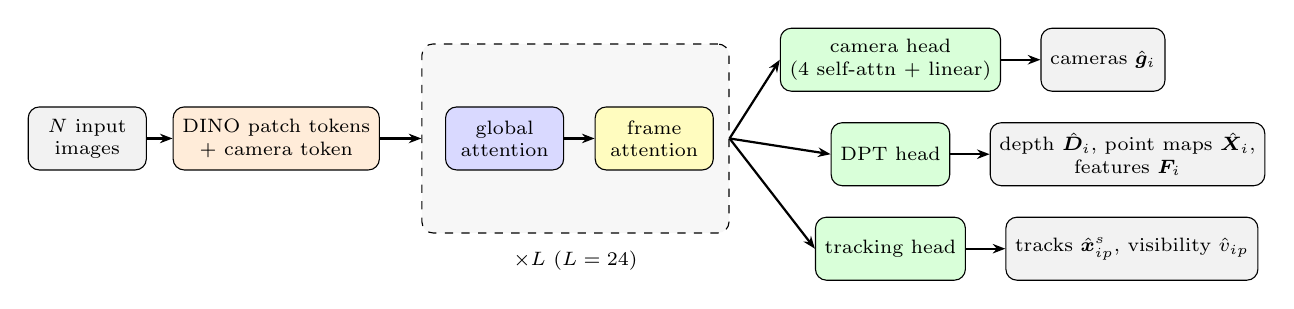
\begin{tikzpicture}[node distance=0.4cm,every node/.style={font=\scriptsize},
 b/.style={draw,rounded corners,minimum height=0.8cm,align=center},
 arr/.style={-{Stealth[length=1.6mm]},thick}]
\node[b,fill=gray!10,minimum width=1.5cm] (in) at (0,0) {$N$ input\\ images};
\node[b,fill=orange!15,minimum width=1.8cm] (tok) at (2.4,0) {DINO patch tokens\\ + camera token};
\begin{scope}[on background layer]
\node[draw,dashed,rounded corners,fill=gray!6,minimum width=3.9cm,minimum height=2.4cm] (blk) at (6.2,0) {};
\end{scope}
\node[b,fill=blue!15,minimum width=1.5cm] (ga) at (5.3,0) {global\\ attention};
\node[b,fill=yellow!25,minimum width=1.5cm] (fa) at (7.2,0) {frame\\ attention};
\draw[arr](ga)--(fa);
\node at (6.2,-1.55) {$\times L$ ($L=24$)};
\node[b,fill=green!15,minimum width=1.5cm] (ch) at (10.2,1.0) {camera head\\ (4 self-attn + linear)};
\node[b,fill=green!15,minimum width=1.5cm] (dpt) at (10.2,-0.2) {DPT head};
\node[b,fill=green!15,minimum width=1.5cm] (tr) at (10.2,-1.4) {tracking head};
\node[b,fill=gray!10,right=0.5cm of ch] (o1) {cameras $\hat{\bm g}_i$};
\node[b,fill=gray!10,right=0.5cm of dpt] (o2) {depth $\hat{\bm D}_i$, point maps $\hat{\bm X}_i$,\\ features $\bm F_i$};
\node[b,fill=gray!10,right=0.5cm of tr] (o3) {tracks $\hat{\bm x}^s_{ip}$, visibility $\hat v_{ip}$};
\draw[arr](in)--(tok);\draw[arr](tok)--(blk);
\draw[arr](blk.east)--(ch.west);\draw[arr](blk.east)--(dpt.west);\draw[arr](blk.east)--(tr.west);
\draw[arr](ch)--(o1);\draw[arr](dpt)--(o2);\draw[arr](tr)--(o3);
\end{tikzpicture}
\caption{VGGT architecture (redrawn and simplified from slide 60).}
\end{figure}

\begin{example}{Cost of global versus frame attention}{attncost}
With $N=10$ images and $T=1369$ patch tokens per image there are $NT=13{,}690$ tokens. Global attention scores $(NT)^2\approx1.87\cdot10^8$ token pairs per head and layer; frame attention scores $N\cdot T^2\approx1.87\cdot10^7$. Frame attention is $N=10$ times cheaper.
\end{example}

\begin{intuition}
Global attention is where views ``talk'' to each other (it learns correspondence and relative pose implicitly); frame attention lets each image digest its own content cheaply. Alternating the two $24$ times mimics what SfM does iteratively (match, then triangulate and refine), but inside one differentiable network with no hand-set thresholds. The camera token acts as a learned ``summary slot'' per image from which the camera is read out; no temporal order is assumed, so the images may be an unordered photo collection.
\end{intuition}

\subsection{Prediction Heads and Tracking \slr{61}}
\begin{itemize}
\item \textbf{Camera head:} four self-attention layers and a linear layer turn the camera token of image $i$ into $\hat{\bm g}_i$.
\item \textbf{DPT head,} the Dense Prediction Transformer decoder (Ranftl et al., ICCV 2021), turns tokens back into per-pixel maps: $\hat{\bm D}_i$, $\hat{\bm X}_i$, $\bm F_i$, and confidence maps $\bm C^D_i,\bm C^X_i\in\R^{H\times W}$ that say how much to trust each pixel of $\hat{\bm D}_i$ and $\hat{\bm X}_i$.
\item \textbf{Tracking head,} as in CoTracker2 (a point tracker for videos): given the pixel of a point $p$ in one image, it compares the feature of that pixel with the feature maps $\bm F_i$ of all images, and predicts where the point appears in each image, $\hat{\bm x}^s_{ip}$, and whether it is visible there, $\hat v_{ip}\in[0,1]$.
\end{itemize}

\subsection{Training Objective and Normalization \slr{62}}
The four outputs are trained jointly, against ground truth written without a hat:
\[
\mathcal L=\mathcal L_{\rm camera}+\mathcal L_{\rm depth}+\mathcal L_{\rm pmap}+\lambda\mathcal L_{\rm track},\qquad\lambda=0.05,
\]
\[
\mathcal L_{\rm depth}=\sum_{i=1}^N\bigl\lVert\bm C^D_i\odot(\hat{\bm D}_i-\bm D_i)\bigr\rVert+\bigl\lVert\bm C^D_i\odot(\nabla\hat{\bm D}_i-\nabla\bm D_i)\bigr\rVert-\alpha\log\bm C^D_i .
\]
Here $\odot$ is the per-pixel product, $\nabla$ the image gradient, and $\alpha$ the weight of the term $-\alpha\log\bm C^D_i$, which keeps the confidence from dropping to zero. $\mathcal L_{\rm camera}$ is a Huber loss, squared for small errors and linear for large ones, between $\hat{\bm g}_i$ and $\bm g_i$; $\mathcal L_{\rm pmap}$ is like $\mathcal L_{\rm depth}$ for $\hat{\bm X}_i$ with $\bm C^X_i$; $\mathcal L_{\rm track}$ is the distance of $\hat{\bm x}^s_{ip}$ to the true positions, plus a visibility term.

\begin{intuition}
The confidence $\bm C$ weights each pixel's error: unreliable pixels (sky, reflections, moving objects) can lower their confidence and so pay less. Without the $-\alpha\log\bm C$ term the network could cheat by predicting $\bm C=0$ everywhere. The term charges a price for low confidence, so confidence drops only where errors would be large. The gradient term in the depth loss encourages sharp, correct edges.
\end{intuition}

\begin{proposition}{Why a normalization is required}{normal}
Let $(\bm T_i,\bm X)$ be a ground-truth reconstruction. Any similarity transform of the whole scene, applied consistently to cameras and points, produces the same images (Prop.~\ref{prop:gauge}). A regression target that is not fixed by a convention is therefore not a function of the images.
\end{proposition}
\begin{proof}
If two targets differ by a similarity, they map to identical inputs, so the network would be asked to output two different answers for the same input; the loss-minimizing prediction would blur between them.
\end{proof}

The images do not fix the global frame and scale (5.3). The ground truth is therefore expressed in the frame of camera 1 and divided by $s$, the mean distance of its 3D points to the origin; the network learns to predict in this normalized frame.

\begin{intuition}
It is the neural-network version of the gauge fixing of bundle adjustment: BA fixes the first pose and one distance; VGGT fixes the first pose and the average point distance (``scene scale $=1$''). Every training scene is thus expressed in the same canonical units.
\end{intuition}

\paragraph{Training data and cost.} 17 datasets; 64 A100 GPUs for nine days; 2 to 24 images per scene, at most 518 pixels per side (the slide quotes around 1.5M EUR for this compute).

\subsection{Results: Camera Pose Estimation \slr{63}}
10 random frames per scene; time on one H100 GPU. AUC@30: area under the accuracy curve of the relative rotation and translation errors, up to $30^\circ$. RealEstate10K: walkthrough videos of houses, used for training by none of the methods. CO3Dv2: videos around everyday objects. PixSfM: COLMAP with feature-metric refinement. DUSt3R and MASt3R with global alignment.

\begin{table}[H]
\centering
\begin{tabular}{lccc}
\toprule
Method & RealEstate10K $\uparrow$ & CO3Dv2 $\uparrow$ & Time\\
\midrule
COLMAP + SuperPoint + SuperGlue & 45.2 & 25.3 & $\approx15$\,s\\
PixSfM & 49.4 & 30.1 & $>20$\,s\\
DUSt3R & 67.7 & 76.7 & $\approx7$\,s\\
MASt3R & 76.4 & 81.8 & $\approx9$\,s\\
VGGSfM v2 & 78.9 & 83.4 & $\approx10$\,s\\
VGGT, feed-forward & 85.3 & 88.2 & $\approx0.2$\,s\\
VGGT + bundle adjustment & \textbf{93.5} & \textbf{91.8} & $\approx1.8$\,s\\
\bottomrule
\end{tabular}
\caption{Camera pose estimation, AUC@30 (slide 63).}
\end{table}

\begin{intuition}
Ten random frames is a sparse, wide-baseline setting, the weakest regime of classical SfM (few overlaps, little parallax per pair). That is where a learned prior helps most: COLMAP+SuperPoint+SuperGlue gets 45.2 on RealEstate10K, VGGT 85.3 in a fifth of a second. On dense captures with thousands of images, incremental SfM remains the reference (5.4). The speed difference ($0.2$\,s versus $\sim15$\,s) is a factor of about 75.
\end{intuition}

\subsection{Results: Dense Geometry \slr{64}}
DTU (lecture 04), Chamfer distance in mm (lower is better); GeoMVSNet is a learned MVS method given the true cameras.

\begin{table}[H]
\centering
\begin{tabular}{@{}lcc@{\hspace{2.2cm}}lc@{}}
\toprule
\multicolumn{3}{c}{DTU} & \multicolumn{2}{c}{ETH3D (laser-scanned GT)}\\
\cmidrule(r{1.2cm}){1-3}\cmidrule{4-5}
Method & GT cameras & Overall$\downarrow$ & Method & Overall$\downarrow$\\
\midrule
GeoMVSNet & yes & 0.295 & DUSt3R & 1.005\\
MASt3R & yes & 0.374 & MASt3R & 0.826\\
DUSt3R & no & 1.741 & VGGT, point head & 0.709\\
VGGT & no & 0.382 & VGGT, depth + camera & \textbf{0.677}\\
\bottomrule
\end{tabular}
\caption{Dense geometry (slide 64).}
\end{table}

\begin{itemize}
\item Depth unprojected with the predicted cameras beats the point head: the decomposition into depth and camera pays off.
\item VGGT obtains dense depth without known cameras, whereas COLMAP's MVS needs SfM first (5.4); on DTU, VGGT (no GT cameras) is within $0.01$\,mm of MASt3R, which \emph{uses} the true cameras.
\end{itemize}
\imgph[4.5cm]{64}{Input, VGGT (``Ours'') and DUSt3R: one image, two images without overlap, 32 images (reconstruction times shown on the slide).}

\subsection{Results: Matching and Tracking \slr{65}}
ScanNet-1500: 1500 indoor image pairs; pose from the matches through the essential matrix (5.3); AUC of the pose error.

\begin{table}[H]
\centering
\begin{tabular}{lccc}
\toprule
Method & AUC@5$^\circ$ & AUC@10$^\circ$ & AUC@20$^\circ$\\
\midrule
SuperGlue & 16.2 & 33.8 & 51.8\\
LoFTR & 22.1 & 40.8 & 57.6\\
RoMa & 31.8 & 53.4 & 70.9\\
VGGT & \textbf{33.9} & \textbf{55.2} & \textbf{73.4}\\
\bottomrule
\end{tabular}
\caption{Two-view matching, pose from the essential matrix (slide 65).}
\end{table}
RoMa is a dense learned matcher and the strongest baseline. The tracking head is \emph{not trained} for two-view matching. The features also serve other tasks: a dynamic point tracker improves when given them, and novel view synthesis works without the input cameras.

\begin{intuition}
It is a surprising result: a network trained for 3D reconstruction produces features that outperform dedicated two-view matchers, because ``being the same 3D point'' is a stronger training signal than ``looking alike''. Note how the pipeline of Section 5.3 (matches $\to$ $\E$ $\to$ pose) is used here as an \emph{evaluation protocol}, which shows the classical geometry remains the common language.
\end{intuition}
\imgph[4.4cm]{65}{Point tracking: VGGT tracks (top) and a dynamic point tracker (CoTracker) given VGGT features (bottom) (Wang et al., CVPR 2025).}

\subsection{Bundle Adjustment from VGGT Predictions \slr{66}}
Use the same objective as before,
\[
\mathcal T^*,\mathcal X_w^*=\argmin_{\mathcal T,\mathcal X_w}\sum_{i=1}^N\sum_{p=1}^P w_{ip}\bigl\lVert\bm x^s_{ip}-\pi_i(\bm x^w_p)\bigr\rVert_2^2,
\]
with the following ingredients, all predicted:
\begin{itemize}
\item observations $\bm x^s_{ip}$ and weights $w_{ip}$: tracks and visibilities from the tracking head;
\item initial poses $\bm T_i$: the camera head, $\hat{\bm g}_i$, which also gives the calibrations $\bm K_i$;
\item initial points $\mathcal X_w$: the predicted depth maps $\hat{\bm D}_i$, unprojected with the predicted cameras.
\end{itemize}
Initialization, image registration and triangulation (5.4) are no longer needed; with bundle adjustment the reconstruction takes about 2\,s. AUC@30 on RealEstate10K rises from 85.3 to 93.5 with bundle adjustment.

\begin{intuition}
The two worlds complement each other: the network gives a very good starting point in the right basin of attraction (solving the non-convexity problem of Section 5.4), and BA then enforces what the network cannot guarantee, namely that the output is \emph{exactly} geometrically consistent with the observed tracks. This is the same ``closed-form initialization + non-linear refinement'' pattern as in Zhang's calibration.
\end{intuition}

\subsection{Limitations \slr{67}}
\textbf{Stated in the paper:}
\begin{itemize}
\item no fisheye or panoramic images;
\item accuracy drops under extreme rotations between the input images;
\item minor non-rigid motion is handled, substantial non-rigid deformation fails;
\item runtime and memory grow with the number of frames: 200 frames take 8.75\,s and 40.63\,GB of GPU memory (one H100, images of $336\times518$ pixels).
\end{itemize}
\textbf{Beyond the paper:}
\begin{itemize}
\item training needs large 3D-labeled datasets and large compute: 17 datasets, 64 A100 GPUs for nine days;
\item no geometric guarantee: the output is a prediction, not the optimum of an objective;
\item bundle adjustment still improves the result: 85.3 to 93.5 AUC@30 on RealEstate10K.
\end{itemize}

\subsection{Comparison of Incremental and Feed-Forward SfM \slr{68}}
\begin{table}[H]
\centering
\small
\begin{tabular}{@{}p{2.6cm}p{5.8cm}p{5.8cm}@{}}
\toprule
 & Incremental SfM & VGGT\\
\midrule
Camera model & perspective, calibrated or self-calibrated & perspective, principal point at the center\\
Views & one at a time & all jointly\\
Assumptions & overlap and texture, a good initial pair & scenes like the training data, mostly rigid\\
Solution & RANSAC and nonlinear least squares & one forward pass of a transformer\\
Runtime & minutes to hours & under a second for tens of frames\\
Scale & thousands of images & hundreds of frames, bounded by GPU memory\\
Output & sparse points and cameras; dense with MVS & cameras, depth, point maps, tracks\\
Failure modes & low overlap, little texture, drift & fisheye images, extreme rotations, non-rigid motion\\
Guarantees & local optimum of the reprojection error & none\\
\bottomrule
\end{tabular}
\caption{Incremental SfM (Sch\"onberger and Frahm, CVPR 2016) versus VGGT (Wang et al., CVPR 2025), slide 68.}
\end{table}

\begin{intuition}
The two are complementary rather than competing: use the feed-forward network when views are few, wide-baseline or the time budget is tight (robots, interactive tools), and use classical incremental or global SfM when you have thousands of images and need a certified, repeatable optimum. The hybrid VGGT + BA gives the best accuracy.
\end{intuition}

%%%%%%%%%%%%%%%%%%%%%%%%%%%%%%%%%%%%%%%%%%%%%%%%%%%%%%%%%%%%%%%%%%%%%%
\section*{Summary \slr{69}}
\addcontentsline{toc}{section}{Summary \emph{(slide 69)}}

\subsection*{Comparison of the methods covered}
\begin{table}[H]
\centering
\small
\begin{tabular}{@{}p{2.9cm}p{3.5cm}p{4.0cm}p{3.1cm}@{}}
\toprule
Method & Input $\to$ output & Core idea & Main limitation\\
\midrule
Zhang calibration (5.1) & plane images $\to$ $\bm K$, poses & homography constraints on $\bm B$, then non-linear LS & needs a known target\\
SIFT (5.2) & image $\to$ 128D features & DoG extrema in scale space, gradient histograms & hand-crafted; slow\\
SuperPoint (5.2) & image $\to$ keypoints + 256D descriptors & self-supervised, homographic adaptation & fails for rotations not in training data\\
8-point / 5-point (5.3) & $\ge8$ / $5$ matches $\to$ $\E$ & linear epipolar constraint (+ rank-2 projection) & scale unobservable; 4-fold ambiguity\\
Triangulation (5.3) & 2 views $\to$ 3D point & DLT or reprojection error & ill-conditioned for small parallax\\
Bundle adjustment (5.4) & observations $\to$ poses, points & Gauss--Newton on $\SE$ + Schur complement & needs good initialization\\
Incremental SfM / COLMAP (5.4) & image set $\to$ sparse model & seed from two views, register, triangulate, BA & slow; drift; many thresholds\\
VGGT (5.5) & $N$ images $\to$ cameras, depth, points, tracks & alternating attention, trained on 17 datasets & no guarantees; GPU memory\\
VGGT + BA (5.5) & $N$ images $\to$ refined model & learned initialization + BA & extra $\sim1.6$\,s\\
\bottomrule
\end{tabular}
\caption{Summary of the methods of Lecture 05.}
\end{table}

\begin{figure}[H]
\centering
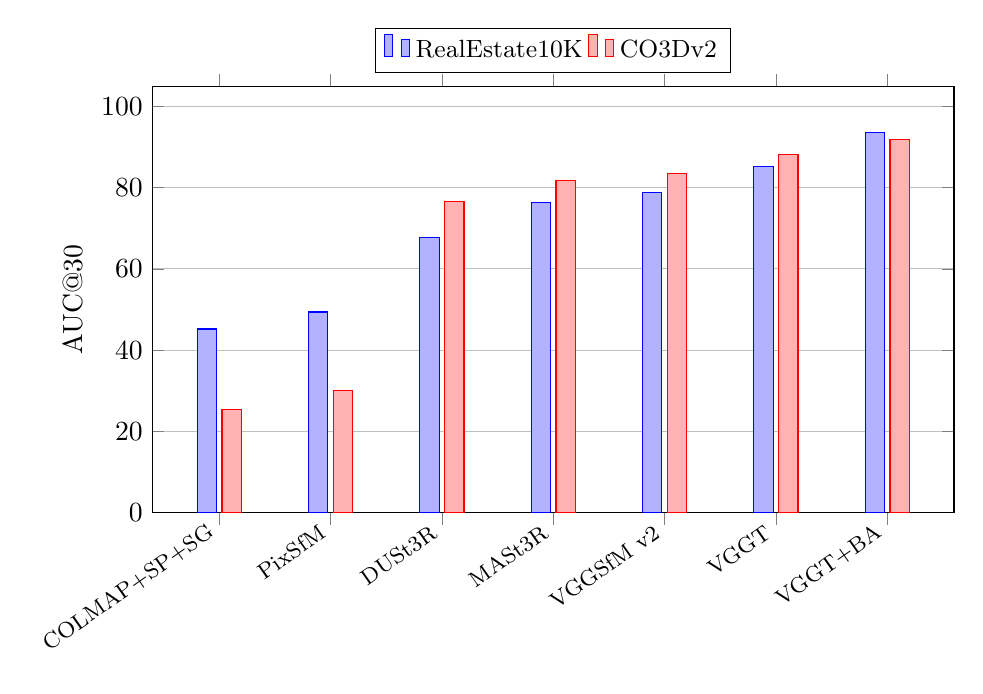
\begin{tikzpicture}
\begin{axis}[ybar,width=0.97\linewidth,height=7cm,bar width=7pt,ymin=0,ymax=105,
 symbolic x coords={c1,c2,c3,c4,c5,c6,c7},xtick=data,
 xticklabels={COLMAP+SP+SG,PixSfM,DUSt3R,MASt3R,VGGSfM v2,VGGT,VGGT+BA},
 xticklabel style={rotate=35,anchor=east,font=\footnotesize},
 legend style={at={(0.5,1.03)},anchor=south,legend columns=2,font=\small},
 ylabel={AUC@30},enlarge x limits=0.1,ymajorgrids]
\addplot coordinates {(c1,45.2)(c2,49.4)(c3,67.7)(c4,76.4)(c5,78.9)(c6,85.3)(c7,93.5)};
\addplot coordinates {(c1,25.3)(c2,30.1)(c3,76.7)(c4,81.8)(c5,83.4)(c6,88.2)(c7,91.8)};
\legend{RealEstate10K,CO3Dv2}
\end{axis}
\end{tikzpicture}
\caption{Camera pose accuracy of classical, learned two-view, and feed-forward methods (data of the table on slide 63; ten random frames per scene). The jump from the classical pipeline to learned methods is largest in the sparse regime, and bundle adjustment on top of VGGT adds the final gain.}
\end{figure}

\subsection*{Key take-aways}
\begin{enumerate}
\item \textbf{Geometry supplies the constraints:} the epipolar constraint, triangulation and the reprojection error are the common language of every method in this lecture, classical or learned (even VGGT is evaluated and refined with them).
\item \textbf{Classical SfM = robust estimation + non-linear least squares.} Sparsity and the Schur complement keep bundle adjustment tractable (a factor $\sim10^8$ in our example); its hard part is the initialization, which is why reconstruction is built incrementally from a good seed.
\item \textbf{Scale and gauge are never observable from images alone:} the essential matrix is defined up to scale and the four-fold decomposition ambiguity is resolved by cheirality; BA fixes one pose and one distance; VGGT normalizes its training targets.
\item \textbf{VGGT learns the whole mapping} from images to cameras, depth, point maps and tracks in one forward pass of a transformer with alternating global and frame attention.
\item \textbf{The most accurate poses come from a learned initialization refined by bundle adjustment} (AUC@30: $85.3\to93.5$ on RealEstate10K).
\end{enumerate}

\vfill
\noindent\small\emph{Acknowledgments (slide 70): the slides are adapted from the Computer Vision course at the University of T\"ubingen (Prof.\ Andreas Geiger); Section 5.5 figures and results are from Wang et al., ``VGGT: Visual Geometry Grounded Transformer'', CVPR 2025.}

\end{document}